\documentclass [a4paper]{article}
\usepackage[utf8]{inputenc}
\usepackage[T1]{fontenc}

%Page margins, header and footer positions
\usepackage{geometry}
 \geometry{
 a4paper,
 total={210mm,297mm},
 left=25mm,
 right=25mm,
 top=30mm,
 bottom=25mm,
 headsep=7mm}

\interfootnotelinepenalty=10000

%To display filling dots in the TOC for all entries
\usepackage[titles]{tocloft}
\renewcommand{\cftsecleader}{\cftdotfill{\cftdotsep}}

%Define new header and footer style
\usepackage{fancyhdr}

\pagestyle{fancy}
\fancyhf{}
\lhead{\color{Gray}{\small{Best Bike Paths project by Alessandro Barbera, Nicolas Bolanos, Massimiliano Nuzzo}}}
\lfoot{\textcolor{Gray}{\small{Copyright © 2026, Alessandro Barbera, Nicolas Bolanos, Massimiliano Nuzzo – All rights reserved}}}
\rfoot{\textcolor{Gray}{\thepage}}
\renewcommand{\headrulewidth}{0pt}

%PACKAGES
\usepackage{wasysym}
\usepackage{pifont}

\newcommand{\supported}{\ding{52}\xspace}
\newcommand{\unsupported}{\ding{55}\xspace}
\newcommand{\partsupported}{\textcolor{black!40}{\ding{52}}\xspace}
\newcommand{\lowsupported}{\textcolor{black!20}{\ding{52}}\xspace}
\newcommand{\unknowsupported}{\textbf{?}\xspace}

%Font: Times
\usepackage{times}
%Change monospaced font
\renewcommand{\ttdefault}{lmtt}

%tables
\usepackage{tabu}
\usepackage{tabularx}
\usepackage{ltablex}
\usepackage{longtable}
\usepackage{float} % To allow the use of H modifier in long tables

%landscape mode
\usepackage{pdflscape}
\usepackage{rotating}
\usepackage{caption}

%make landscape mode be sensitive to even and odd pages
%start
\def\myrotate{\ifodd\c@page\else-\fi 90}
\makeatletter
\global\let\orig@begin@landscape=\landscape%
\global\let\orig@end@landscape=\endlandscape%
\gdef\@true{1}
\gdef\@false{0}
\gdef\landscape{%
    \global\let\within@landscape=\@true%
    \orig@begin@landscape%
}%
\gdef\endlandscape{%
    \orig@end@landscape%
    \global\let\within@landscape=\@false%
}%
\@ifpackageloaded{pdflscape}{%
    \gdef\pdf@landscape@rotate{\PLS@Rotate}%
}{
    \gdef\pdf@landscape@rotate#1{}%
}
\let\latex@outputpage\@outputpage
\def\@outputpage{
    \ifx\within@landscape\@true%
        \if@twoside%
            \ifodd\c@page%
                \gdef\LS@rot{\setbox\@outputbox\vbox{%
                    \pdf@landscape@rotate{-90}%
                    \hbox{\rotatebox{90}{\hbox{\rotatebox{180}{\box\@outputbox}}}}}%
                }%
            \else%
                \gdef\LS@rot{\setbox\@outputbox\vbox{%
                    \pdf@landscape@rotate{+90}%
                    \hbox{\rotatebox{90}{\hbox{\rotatebox{0}{\box\@outputbox}}}}}%
                }%
            \fi%
        \else%
            \gdef\LS@rot{\setbox\@outputbox\vbox{%
                \pdf@landscape@rotate{+90}%
                \hbox{\rotatebox{90}{\hbox{\rotatebox{0}{\box\@outputbox}}}}}%
            }%
        \fi%
    \fi%
    \latex@outputpage%
}
\makeatother
%end

%graphics
\usepackage{graphicx}
\usepackage[dvipsnames, table]{xcolor}
%If you upload images from PC, you need to insert code for the path here (different for Windows and Unix OS)

%References
%\usepackage{xpatch}
%\usepackage[backend=biber, style=numeric, citestyle=numeric, sorting=none]{biblatex}
%\addbibresource{main.bib}

%Other
\usepackage{ifthen}
\usepackage{xspace}
\usepackage{enumitem}
\usepackage{amssymb}
\usepackage{listings}
\usepackage[colorlinks=true, linkcolor=black]{hyperref}
\newcommand{\comment}[1]{{\color{Red}$\blacktriangleright$ Comment: #1 $\blacktriangleleft$}}


\setlength{\parskip}{\baselineskip}

% Some utilities\ldots
\usepackage{soul}
\usepackage{tikz}

\usetikzlibrary{calc}
\usetikzlibrary{decorations.pathmorphing}


\makeatletter

\newcommand{\defhighlighter}[3][]{%
  \tikzset{every highlighter/.style={color=#2, fill opacity=#3, #1}}%
}

\defhighlighter{yellow}{.5}

\newcommand{\highlight@DoHighlight}{
  \fill [ decoration = {random steps, amplitude=1pt, segment length=15pt}
        , outer sep = -15pt, inner sep = 0pt, decorate
       , every highlighter, this highlighter ]
        ($(begin highlight)+(0,8pt)$) rectangle ($(end highlight)+(0,-3pt)$) ;
}

\newcommand{\highlight@BeginHighlight}{
  \coordinate (begin highlight) at (0,0) ;
}

\newcommand{\highlight@EndHighlight}{
  \coordinate (end highlight) at (0,0) ;
}

\newdimen\highlight@previous
\newdimen\highlight@current

\DeclareRobustCommand*\highlight[1][]{%
  \tikzset{this highlighter/.style={#1}}%
  \SOUL@setup
  %
  \def\SOUL@preamble{%
    \begin{tikzpicture}[overlay, remember picture]
      \highlight@BeginHighlight
      \highlight@EndHighlight
    \end{tikzpicture}%
  }%
  %
  \def\SOUL@postamble{%
    \begin{tikzpicture}[overlay, remember picture]
      \highlight@EndHighlight
      \highlight@DoHighlight
    \end{tikzpicture}%
  }%
  %
  \def\SOUL@everyhyphen{%
    \discretionary{%
      \SOUL@setkern\SOUL@hyphkern
      \SOUL@sethyphenchar
      \tikz[overlay, remember picture] \highlight@EndHighlight ;%
    }{%
    }{%
      \SOUL@setkern\SOUL@charkern
    }%
  }%
  %
  \def\SOUL@everyexhyphen##1{%
    \SOUL@setkern\SOUL@hyphkern
    \hbox{##1}%
    \discretionary{%
      \tikz[overlay, remember picture] \highlight@EndHighlight ;%
    }{%
    }{%
      \SOUL@setkern\SOUL@charkern
    }%
  }%
  %
  \def\SOUL@everysyllable{%
    \begin{tikzpicture}[overlay, remember picture]
      \path let \p0 = (begin highlight), \p1 = (0,0) in \pgfextra
        \global\highlight@previous=\y0
        \global\highlight@current =\y1
      \endpgfextra (0,0) ;
      \ifdim\highlight@current < \highlight@previous
        \highlight@DoHighlight
        \highlight@BeginHighlight
      \fi
    \end{tikzpicture}%
    \the\SOUL@syllable
    \tikz[overlay, remember picture] \highlight@EndHighlight ;%
  }%
  \SOUL@
}

\makeatother

% Common abbrev. are set as commands to ensure proper spacing after the dot
\RequirePackage{xspace}
\newcommand{\ie}{i.e.\@\xspace}
\newcommand{\aka}{a.k.a.\@\xspace}
\newcommand{\Ie}{I.e.\@\xspace}
\newcommand{\cf}{cf.\@\xspace}
\newcommand{\Cf}{Cf.\@\xspace}
\newcommand{\eg}{e.g.\@\xspace}
\newcommand{\Eg}{E.g.\@\xspace}
\newcommand{\etal}{et al.\@\xspace}
\newcommand{\etc}{etc.\@\xspace}
\newcommand{\wrt}{w.r.t.\@\xspace}
\newcommand{\Wrt}{W.r.t.\@\xspace}



\date{}

\usepackage{wrapfig}
\usepackage{multicol}
\usepackage{longtable}

\definecolor{alloygreen}{rgb}{0,0.6,0}
\definecolor{alloyblue}{rgb}{0,0,0.6}
\definecolor{alloygray}{rgb}{0.5,0.5,0.5}

\lstdefinestyle{alloy}{
  basicstyle=\ttfamily\footnotesize,
  keywordstyle=\color{alloyblue},
  commentstyle=\color{alloygreen},
  numbers=left,
  numberstyle=\tiny\color{alloygray},
  breaklines=true,
  showstringspaces=false,
  keepspaces=true,
  frame=lines,
  morecomment=[l]{//},
  morecomment=[s]{/*}{*/},
  morekeywords={
      abstract, sig, extends,
      one, lone, some, set,
      fact, all, no, in, not,
      pred, fun, run, check, for,
      open, module, but
  }
}


\begin{document}

%TITLE PAGE

\begin{titlepage}

%LOGO

{\begin{table}[t!]
\centering
\begin{tabu} to \textwidth { X[1.3,r,p] X[1.7,l,p] }
\textcolor{Blue}
{\textbf{\small{}}} & 
\includegraphics[scale=0.5]{Images/PolimiLogo}
\end{tabu}
\end{table}}~\\ [7cm]

%TITLE 

\begin{flushleft}

%Replace the text string with your title
{\textcolor{Blue}{\textbf{\Huge{Requirement Analysis and Specification
        Document}}}} \\ [1cm]

\end{flushleft}

\end{titlepage}

%Define deliverable specific info
%Replace cell contents where needed
\begin{table}[h!]
\begin{tabu} to \textwidth { X[0.3,r,p] X[0.7,l,p] }
\hline

\textbf{Deliverable:} & RASD\\
\textbf{Title:} & Requirement Analysis and Specification Document \\
\textbf{Authors:} & Alessandro Barbera, Nicolas Bolanos, Massimiliano Nuzzo \\
\textbf{Version:} & 1.0 \\ 
\textbf{Date:} & 23-December-2025 \\
\textbf{Download page:} & https://github.com/nicolasbolanospolimi/BarberaBolanosNuzzo \\
\textbf{Copyright:} & Copyright © 2026, Alessandro Barbera, Nicolas Bolanos, Massimiliano Nuzzo – All rights reserved \\
\hline
\end{tabu}
\end{table}


\setcounter{page}{2}


%------------------------------------------------------------------------------------------------------------------------------------------------
\newpage
\addcontentsline{toc}{section}{Table of Contents}
\tableofcontents
\newpage
\addcontentsline{toc}{section}{List of Figures}
\listoffigures
\addcontentsline{toc}{section}{List of Tables}
\listoftables

%------------------------------------------------------------------------------------------------------------------------------------------------
\clearpage
{\color{Blue}{\section{Introduction}}}
\label{sect:introduction}

\subsection{Purpose}

Cycling is not always the safest activity, the cyclist does not always have a dedicated infrastructure and sometimes must share among other road actors. Also, people are not always aware of the existence of paths, or roads that are in better condition than other when going from one place to another. In order to make biking a more efficient and safe, both as a sporting activity and mean of transport, Best Bike Paths (BBP) is created. 

BBP aims to promote safer, more efficient, and enjoyable cycling by enabling users to discover and evaluate bike routes based on path conditions, obstacles, and user feedback. BBP supports active contribution and collaboration from cyclists, allowing them to record their trips, share path conditions, and confirm or correct automatically collected data, fostering a community-driven platform that keeps information current and reliable.

BBP encourages sustainable urban mobility by motivating more people to cycle through improved route transparency and safety awareness. It also helps local authorities and communities by aggregating data to identify needed maintenance or hazards on bike paths, potentially contributing to better infrastructure planning and maintenance. 

\subsubsection{Goals}
\textbf{G1:} Users can register and have a profile in BBP application.\\
\textbf{G2:} Users manually create bike paths in an inventory by specifying the name of the streets and the status.\\
\textbf{G3:} Users create bike paths in an automated mode where the system acquire data from the user's mobile device and reconstruct the path.\\
\textbf{G4:} Users browse bike paths within the inventory. They can specify an origin and destination and ask the system to visualize the bike path on a map. \\
\textbf{G5:} Users record their trips and store them to keep track of their cycling activities.\\
\textbf{G6:} Users can see for a recorded trip various statistical data of the user performances as well as meteorological information during the respective trip.\\
\textbf{G7:} The system uses information published by the users about the paths by merging pieces of information to generate the optimal path, using the freshness and number of confirmed data.\\

\subsection{Scope}

The core goal is to help cyclists easily discover and evaluate paths based on user-contributed trip data, path conditions, and obstacles. BBP enables both registered and unregistered users to explore and access reliable data about cycling paths based on their quality, safety, and efficiency. 

BBP allows users to contribute information about bike paths either manually or automatically. In manual mode, users enter data such as street names, surface conditions, and obstacles. In automatic mode, BBP leverages mobile device sensors, including GPS, accelerometers, and gyroscopes, to detect paths and irregularities during rides. The system filters these inputs for accuracy through user confirmation before making them public.

BBP also aggregates and merges data from multiple contributors, giving preference to the most recent and widely confirmed information helping to keep the bike path inventory up-to-date and relevant for all users. 

Also, registered users can record their individual trips, obtaining detailed statistics such as total distance, average speed, and travel duration. The system also integrates meteorological data from external services, enriching trip records with real-time weather conditions like temperature, wind speed, and precipitation.

Ultimately, the system aims to enhance cycling safety, promote community engagement, sport activities on the bike, and support sustainable mobility by providing up-to-date, user-verified information about the best available bike paths. 

%------------WORLD PHENOMENA---------------------
\subsubsection{World Phenomena}

\begin{enumerate}[label=\textbf{WP\arabic*:}]
    \item Users ride bikes in paths. 
    \item Users choose specific paths to ride.
    \item Weather conditions affects visibility and riding performance of riders.
    \item Physical obstacles on the path may be encountered, which may affect users by continuing the riding.
    \item External services provides information about the weather forecasting.
    \item Road go under maintenance in certain periods.
    \item Road gets closed for certain events.
    \item Road gets modified.
    \item Road gets permanently closed.
    \item Road deteriorates over time.
\end{enumerate}
%------------SHARED PHENOMENA---------------------
\subsubsection{Shared Phenomena}
\begin{enumerate}[label=\textbf{SP\arabic*:}]
    \item (If automatic mode enabled) The system collects the information from the registered user traversing paths.
    \item (If automatic mode enabled) Registered user confirms path information.
    \item (If automatic mode disabled) Registered User provides path information manually.
    \item User search for paths.
    \item Registered user publishes a new path.
    \item Registered user updates a road status.
    \item (If automatic mode enabled) Registered user starts riding.
    \item (If automatic mode enabled) Registered user stops riding.
    \item Registered user enables automatic mode.
    \item Registered user disables automatic mode.
    \item Registered user start recording a trip.
    \item Registered user stops recording a trip
\end{enumerate}

\subsection{Definitions, Acronyms, Abbreviations}

\subsubsection{Definitions}

\begin{itemize}
    \item \textbf{Registered User}: A person who creates an account in the BBP system to access advanced features such as recording and publishing trips, adding or confirming path information, and contributing data either manually or automatically.
    \item \textbf{Path}: A cycling route between a starting and finishing point recorded in the system. It consists of one or more streets or segments where bicycles can circulate under suitable conditions. Each path has associated information about its status, obstacles, and overall score. This score is computed based on the status of the path and on how effective the path is to let the user reach the destination from the given origin.
    \item \textbf{Trip}: An individual cycling activity performed by a registered user. It includes data such as total distance, average speed, duration, and, when available, weather information related to the ride.
    \item \textbf{External Service}: A data source outside the BBP system used to enrich trip information, particularly regarding weather conditions such as temperature, wind speed, and general climate.
    \item \textbf{Automatic Mode}: A data insertion mode in which BBP automatically collects information from the user’s mobile device during the ride. It uses GPS, accelerometer, and gyroscope data to reconstruct the followed path and detect irregularities such as potholes, which the user must later confirm or correct.
    \item \textbf{Manual Mode}: A data insertion mode in which the user manually inputs information about a path, specifying streets, path conditions, and any relevant obstacles or issues observed during the ride.
\end{itemize}

\subsubsection{Acronyms}

\begin{itemize}
    \item \textbf{BBP}: Best Bike Paths
    \item \textbf{SDK}: Software Development Kit
    \item \textbf{DBMS}: Database Management System
    \item \textbf{GPS}: Global Positioning System
    \item \textbf{WRS}: Weather Reporting System
\end{itemize}

\subsubsection{Abbreviations}

\begin{itemize}
    \item \textbf{G}: Goal
    \item \textbf{WP}: World Phenomena
    \item \textbf{SP}: Shared Phenomena

\end{itemize}

\subsection{Revision History}

\begin{itemize}
    \item 23/12/2025 - Version 1.0:
        \begin{itemize}[label=+]
            \item Added Section 1
            \item Added Section 2
            \item Added Section 3
            \item Added Section 4
        \end{itemize}
    \item 07/01/2026 - Version 2.0
        \begin{itemize}[label=+]
            \item Updated Domain Class Diagram: added fields to Trip Class regarding longitude and latitude
            \item Updated order of execution of Login: now we check before for the verification and later for the credentials
            \item Changed functional requirement phrasing: now the path information in automated mode is not saved "locally"
        \end{itemize}
\end{itemize}

\subsection{Reference Documents}

The assignment for this document and all the information included refer to the following documentation:

\begin{itemize}
    \item The specification for the 2025/26 Requirement Engineering and Design Project for the Software Engineering II course.
    \item The slides on the webeep page of the Software Engineering II course.
\end{itemize}

\subsection{Document Structure}

\begin{enumerate}
    \item \textbf{Introduction}: a brief description of the project that follows from the analysis of the specification provided, it highlights the goals of the product and its scope.
    \item \textbf{Overall Description}: a more detailed description of the product that comprehends also real world scenarios and analyses the system from a technical point of view.
    \item \textbf{Specific Requirements}: a detailed list of all the requirements needed in order to satisfy the goals, and their relationship with domain assumptions
    \item \textbf{Formal analysis using Alloy}: a formal description of a portion of real world phenomena analyzed through Alloy in order to highlight inconsistencies between assumptions and phenomena previously modelized.
    \item \textbf{Effort spent}: the time spent by each member of the group to contribute to the realization of this document.
    \item \textbf{References}: reference to documents or tools used for writing this document.
\end{enumerate}

%------------------------------------------------------------------------------------------------------------------------------------------------
\clearpage
{\color{Blue}{\section{Overall Description}}}
\label{sect:overview}
\subsection{Product perspective}

\subsubsection{Scenarios}

\subsubsection*{User wants to register with an account to BBP}
A user U wants to join the BBP community. U downloads the app from their favorite AppStore and opens it. U then goes to the registration page, enters their data (Username, Email, Password) and proceeds to the authentication phase. A message is sent to their email address and U must confirm their account. After that, they are ready to log in

\subsubsection*{Registered User wants to log in with their account to BBP}
A registered user RU wants to log into their BBP account. RU opens the application on their smartphone and goes to the Login Page. Here, RU inserts their Username and their Password. BBP will hash the password and try to match the fingerprint with the one associated to RU account. If it is correct, the login process ends. If not, an error message appears and another attempt at login can be done.

\subsubsection*{Registered user enables automated mode}
A registered user RU logs into the BBP application and enables the automated mode in the home page. The application prompts RU into authorizing access to the device's sensors (GPS, accelerometer, and gyroscope) as well as background execution to allow the system to start collecting data from their mobile device. The application then starts monitoring things like speed, vibrations, among other data to determine whether the user is riding a bike or not.

\subsubsection*{Registered user disables automated mode}
A registered user RU disables automated mode. After this action, BBP no longer collects location or sensor data automatically. Future paths must be recorded manually if the user wants to add new ones. The user can re-enable automated mode at any time.

\subsubsection*{Registered user does a bike ride with automated mode}
A registered user RU starts cycling with automated mode enabled. BBP detects the user’s speed and movement, confirming that the user is biking. During the ride, the system collects GPS coordinates and motion sensor data to reconstruct the path and identify possible obstacles. After the sensors detect that RU stopped cycling, BBP starts processing the just collected data and notifies RU (with a pop-up notification on their phone) that the path has been recorded and that needs revision to be published. RU can decide either to review the entry, or to ignore it and delete it.


\subsubsection*{Registered user wants to publish a path recorded in automated mode}
After their cycling activity, a registered user RU wants to publish the recently recorded path, and make it available for every other user. In doing this, they either press the pop-up notification or open the application by pressing the icon. BBP shows them a summary of the path, including detected issues. RU reviews the information, and changes the incorrect or problematic parts (if any). Finally, RU can publish the entry to the application, ready to be used by BBP.

\subsubsection*{Registered user publishes a bike path in manual mode}

A registered user RU accesses the manual entry section in BBP to add a new bike path. RU specifies the streets that compose the path and assigns a status to each road that composes the path. The user adds details like the presence of obstacles and surface type. Once the information is complete and reviewed, RU publishes the path, allowing it to become visible to all the user base.

\subsubsection*{Registered user records a trip}
A registered user RU begins recording a new cycling session using the BBP application. If the access of the sensors (GPS, accelerometer, and gyroscope) and background execution has not been granted yet, the application will prompt the user to allow access. BBP records the trip details through the device's sensors, including: start and end timestamps, total distance covered, and average speed. Upon completion, RU can save the trip to their personal log and view statistics. 
Asynchronously, once the trip is finished, BBP will use a external service that provides weather data to enrich the trip's data with information such as: Temperature, wind speed, and precipitation.

\subsubsection*{User searches for paths}

A user U, whether registered or not, specifies an origin O and destination D. BBP calculates, using the road stored in its database, all the possible bike paths between O and D. If multiple options are available, BBP displays them ranked by their path score, which depends on path status (calculated as a mean of all the statuses of the single roads in the path) and effectiveness. U can visualize the suggested routes on the map and explore details about obstacles and path condition.

\pagebreak
\subsubsection{Domain Class Diagrams} 

\begin{figure}[H]
\centering
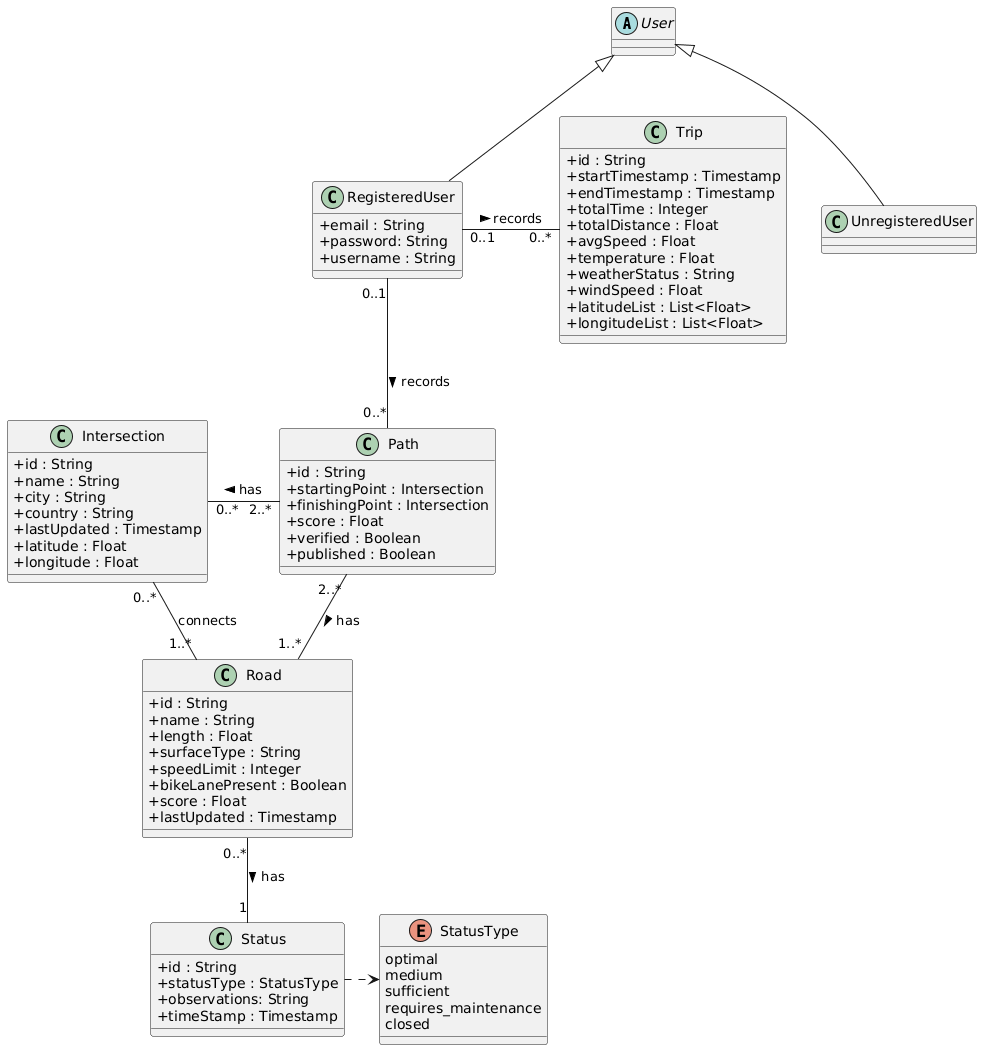
\includegraphics[width=\textwidth]{RASD/Images/Diagrams/Domain/domain-class-3.png}
\caption{\label{fig:domainclass}Domain class diagram for BBP.}
\end{figure}

This Domain Class Diagram ~\cite{uml_diagrams_class_2025} represents the entities involved in the domain of our system and
the relationships between them. Some important points to note:

\begin{itemize}[label=-]
    \item The system distinguishes between registered and unregistered users, with registered users capable of recording trips, contributing data, and making information publishable, while unregistered users can only access information but not contribute or personalize their data.
    \item Registered users can record trips, which include detailed statistics like total time, total distance, average speed, and meteorological data (weather, temperature, wind speed) when available, supporting richer activity logging. 
    \item Paths connect intersections (nodes), utilizing roads as their links, mirroring the real-world and supporting route computation for origin-destination queries. Each path can be marked as verified, published, and scored, facilitating ranking and quality assessment based on both user input and system-calculated factors. Roads and their status types (e.g., optimal, requires maintenance, etc.) allow precise condition reporting, which is crucial for route planning and safety.
    \item The system allows both manual and automated data entry for path and obstacle information, supporting flexibility for user input and leveraging sensor data for finer granularity. Automated mode requires post-capture user verification, addressing the problem of false positives (e.g., erroneous pothole detections), ensuring data quality before publication.
    \item The system supports community-driven data integration, where multiple user contributions about the same path or road are aggregated, prioritizing information based on freshness and majority consensus for better accuracy and reliability. 
    \item Both registered and unregistered users can visualize computed paths based on road status and path effectiveness , helping users choose optimal routes.
\end{itemize}

\newpage

\subsubsection{State Machine Diagrams}~\cite{STM}
\textbf{The registered user records a Trip}
\begin{figure}[H]
    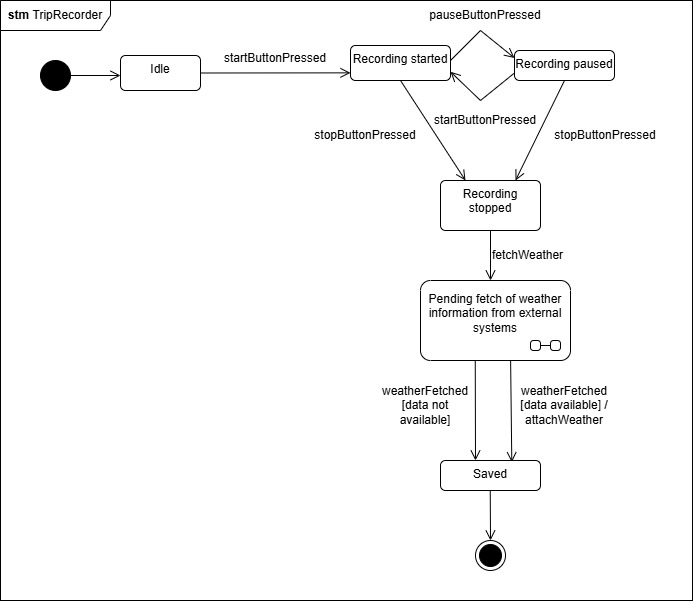
\includegraphics[width=\textwidth]{Images/Diagrams/State Machine/TripRecordingSTM.jpg}
\end{figure}
This state machine describes the different states in which the TripRecorder can be found. At first, the machine is in idle state, waiting for the user to decide if they want to start a recording.\newline
After pressing the start button, the application starts recording, acquiring information on the streets and intersections crossed by the biker, their average speed, max speed, time passed and distance traveled. The user can decide, at any time, to pause and resume the recording while cycling.\newline
At the end of the entire trip, the stop button is pressed and the data is processed.\newline
During data processing, the application asks an external weather reporter system additional data, to enrich trip details. If this information is present, they are attached to the trip recording.\newline
Regardless of the outcome, the trip is saved and now ready to be reviewed.\newline
\newpage

\textbf{The registered user records a Path}
\begin{figure}[H]
    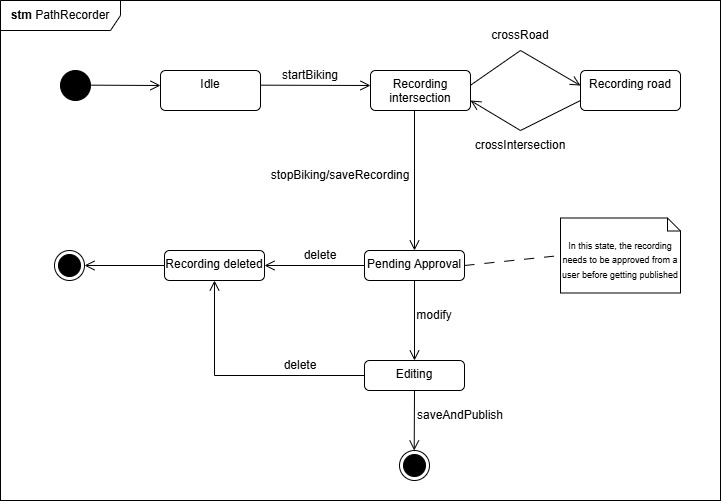
\includegraphics[width=\textwidth]{Images/Diagrams/State Machine/PathRecordingSTM.jpg}
\end{figure}
This state machine describes the different states in which the PathRecorder can be found. Please note that this diagram is showing the \textbf{Automated Mode} only. The \textbf{Manual Mode} is very similar, and journaling is delegated to the user.\newline
After selecting the automated mode in the home page, the machine goes in idle state, waiting for the user to start biking.\newline
When the external sensors (GPS, gyroscope, accelerometer) detect a possible cycling motion, the application starts recording the cycling activity. At this point, roads and intersections information are acquired using the same sensors (especially estimating road conditions and position into the map) until the biker stops cycling.\newline
All the collected data is then saved and ready to be reviewed. Considering the possibility of having false positives, the path must be reviewed by the user before it reaches the published state. In any moment of this process, the path can be discarded and never published.\newline
At the end of the editing phase, the path is saved and published, now available to be used by the application to find paths for other users.
\newpage
\textbf{User searches for Paths}
\begin{figure}[H]
    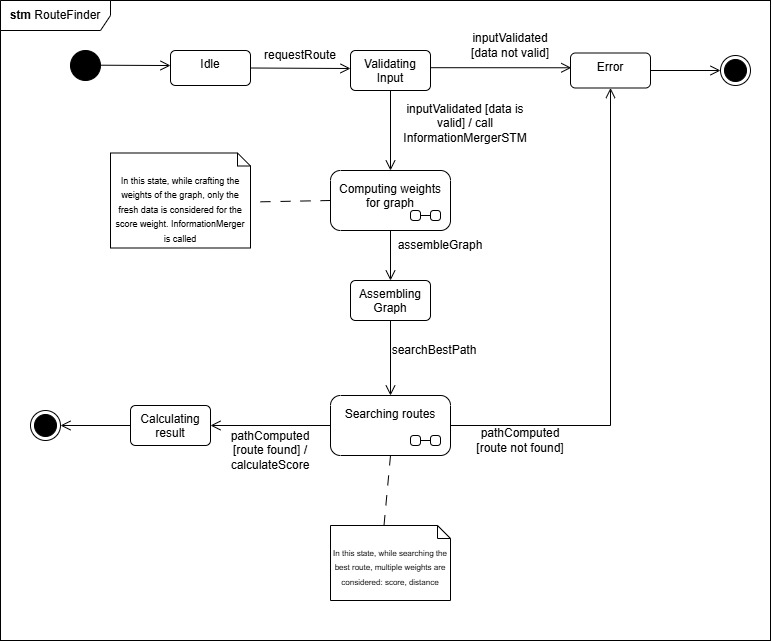
\includegraphics[width=\textwidth]{Images/Diagrams/State Machine/RouteFinderSTM.jpg}
\end{figure}

This state machine describes the different states in which the RouteFinder can be found. This machine is used to calculate the possible routes between a starting point and an ending point selected by the user.\newline
After inserting the start and ending positions, a request to the machine is sent and the input validated. An error occurs if the positions do not exist inside BBP.\newline
The chosen model to represent this problem is a graph, with intersections as nodes and roads as weighted arcs. Please note that, if the starting point is not an intersection but positioned inside the road, an additional parameter is multiplied to the weights to express the real position inside the graph. These weights need to be retrieved from BBP database. In particular, the roads "conditions" could be ambiguous due to multiple entries added at the same time. To solve this issue, the condition weight is calculated by another machine (see  ~\hyperref[fig:informationmerger]{InformationMergerSTM} below) to evaluate the real current condition of the road.\newline
The graph is then built and routes found by using classical route searching algorithms in graphs. For each route, a score is calculated to be correctly displayed in the mobile application.
\newpage

\textbf{The road score is calculated}
\begin{figure}[H]
    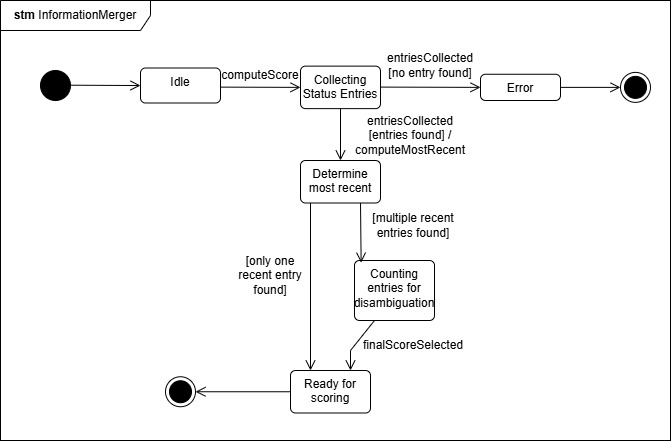
\includegraphics[width=\textwidth]{Images/Diagrams/State Machine/InformationMergerSTM.jpg}
    \label{fig:informationmerger}
\end{figure}

This state machine describes the different state in which the InformationMerger can be found. This machine is used to merge and present the current and most fresh information to the user.\newline
When it is asked to compute a specific road condition, the machine fetches the status entries from the application database regarding that specific road and uses the "timestamp" attribute to determine the most recent entry.\newline
To consider also the possibility of multiple entries with the same timestamp, if the machine finds this "ambiguity", it also performs a "disambiguation" operation: it counts, for every different label of the road condition, the entries with the same timestamp and returns only the one with the biggest cardinality. If even in this case, it's present an ambiguity, it returns the worst label of the group (this guarantees the safety of the biker, avoiding any possible injury).

\subsection{Product functions}

\subsubsection*{Sign Up}

Users can create a new account by providing the necessary personal information to register with the Best Bike Paths (BBP) system. The required personal information includes:
\begin{enumerate}
    \item Username
    \item Email
    \item Password
\end{enumerate}
After submitting the registration form, a confirmation email will be sent to the user's email address. Once the user confirms their account, they will be considered successfully registered and will be redirected to the login page to perform their first login.

\subsubsection*{Login}
The BBP application allows users to sign in using an email address and a password. After inserting the credentials, BBP will check the correctness of the information (f.e. that an email address is associated to an account, or that the account has been successfully verified) and will redirect the user to the home page if that is the case.
If an error during this step has occurred, BBP will notify the user about it.

\subsubsection*{Record a trip}
Registered users can record their cycling activities using the BBP application. When a user starts trip recording, the system collects data from GPS, accelerometers, and gyroscopes to accurately track the route and motion. Upon trip completion, BBP processes the collected data to calculate various statistics, including total distance covered, average speed, and total time spent. The recorded trip is then saved to the user's account and can be viewed through the application interface.

\subsubsection*{Enrich a trip's data}

Once a trip is uploaded to BBP, an asynchronous process begins to enrich the trip data with meteorological information such as weather conditions, temperature, and wind speed. This data is retrieved from an external service and then integrated into the existing trip record. After the trip is updated, users can view the additional meteorological details on the trip detail interface.


\subsubsection*{Insert and publish a bike path}

The BBP application offers two modes for collecting raw data, depending on the user’s preference.\\
\begin{enumerate}
    \item \textbf{Automated Mode}\\
In the automated mode, the BBP application leverages all the built-in sensors of the user’s device to automatically gather the necessary raw data for reconstructing the complete path. Specifically, the GPS sensor is used to track the user’s journey, while motion sensors such as the gyroscope and accelerometer help assess the difficulty of the path at each point—enabling the detection of potholes or other irregularities affecting the ride quality.
To improve the reliability of the collected data, users are encouraged to review and confirm the system’s detections once the journey is completed.
    \item \textbf{Manual Mode} \\
The manual mode is simpler and entirely relies on the user’s honesty and accuracy when entering information. In this case, the user must manually specify the names of the streets included in the path and indicate their respective conditions. If the condition of a path is not "Optimal", the user can also add details about the problems encountered.
\end{enumerate}

\subsubsection*{Browse bike paths}

Any user can explore available bike paths by specifying origin and destination points. The system displays the routes on a map, presenting relevant information such as path conditions, obstacles, and maintenance status to assist in route selection. When multiple paths are available, BBP visualizes them and assigns a score to each, reflecting the quality of the path based on its effectiveness and current condition. This scoring helps users evaluate and choose the most suitable route for their needs.

\subsubsection*{Score a path}

The BBP system collects information from multiple paths and visualizes it through a scoring mechanism. The score is primarily based on the condition of the path and its effectiveness in enabling the user to reach the desired destination from a given origin. The score is given by the user using tags.

\subsubsection*{Merging of similar paths and updating statuses}

When multiple users provide information about the same bike path, BBP merges the data by evaluating the recency of each input and the number of confirming reports. This merging process automatically updates the path’s status to reflect the most accurate, consensus-driven information. Users may tag paths with statuses such as “Optimal” or “Requiring maintenance.” During data consolidation, BBP prioritizes the tag from the most recent input to ensure the path status remains up to date.


\subsection{Users characteristics}

Any user — whether an experienced rider or completely new to biking — can join the platform through the application. Each path shared by a user remains anonymous and is not linked to its creator. As a result, all related paths are automatically collected and anonymously made available to other users. The user is able to insert information, scores of hardness, and any kind of information to any path taken. Furthermore, the user can even relies on the platform to automatically generate the information, however, a final check to the information must be provided. Every user profile and information are private and remain hidden from other users.

\subsubsection{Any user (non-registered and registered users)}

All users, whether registered or not, can explore the information provided by Best Bike Paths (BBP). They can use the map interface to enter an origin and a destination, asking BBP to show possible bike routes between those points. When several options exist, the system ranks them by a score based on path condition, safety, and route effectiveness. \\
Users can view each path’s detailed information, including maintenance status, surface quality, and possible obstacles like potholes. However, unregistered users cannot record trips or add new information, but still access BBP’s main navigation and route-finding tools supported by community data.

\subsubsection{Registered users}

Registered users gain access to extended features supporting individualized interaction and community contribution. They may record personal cycling activities, which are stored within their user profiles and supplemented by metrics such as total distance traveled, average speed, and detailed trip analytics. BBP may augment recorded trips with meteorological data, including weather conditions and temperature, sourced from external services. \\
Furthermore, registered users can contribute path information via two mechanisms: manual and automated. Manual mode allows users to annotate routes with names and assign path statuses. Automated mode enables BBP to collect and analyze path data in real time using mobile device sensors, subsequently allowing users to confirm or revise detected obstacles prior to publication. Validated contributions may be made publishable, with BBP consolidating multiple reports to reflect the most current and consistent community knowledge. These functionalities ensure that registered users can both improve and benefit from the evolving quality of information within the platform.

\subsection{Assumptions, dependencies and constraints}

\subsubsection{Regulatory policies}

The application is designed to enhance the overall user experience by providing an intuitive and efficient interface for data collection and sharing paths. Any user, regardless of their level of experience, can contribute to the platform by recording and publishing biking paths through the application. All related paths are automatically gathered and processed without any association with their original creator, ensuring that personal information remains strictly confidential. This approach guaranties full compliance with the General Data Protection Regulation (GDPR) \cite{gdpr_info_2025} and establishes a secure environment in which users can freely share useful data while maintaining anonymity. Furthermore, personal data are used exclusively for authentication and registration purposes — specifically for log-in via email, account setup, and authorization to access device sensors or third-party services. No personal information is used for any other purpose.

\subsubsection{Domain Assumptions}

\begin{itemize}
    \item \textbf{D1}: Each user rides a bicycle while the application runs in background in case of automated mode.
    \item \textbf{D2}: The internet connection remains relatively stable throughout the session.
    \item \textbf{D3}: Users are willing to review and refine the automatically collected information gathered by the device in the automated-mode.
    \item \textbf{D4}: Users are expected to provide accurate and non-misleading information when creating new paths.
    \item \textbf{D5}: Users do not use the application or the platform for purposes unrelated to biking activities or the exploration of new routes as a recreational activity.
    \item \textbf{D6}: Third-parties services provide reliable information to the application.
    \item \textbf{D7}: Hardware devices must provide reliable sensor data to the system to let it acquire the right performance data.
    \item \textbf{D8}: The date related to the new inserted path is correct.
    \item \textbf{D9}: The app is used where bike track already exists.
    \item \textbf{D10}: The biking paths have little to no cars presence.
    \item \textbf{D11}: The biking paths have speed limits compatible with the average speed of a bike.
    \item \textbf{D12}: Users will stop cycling when they want to end the recording of the path.
    \item \textbf{D13}: Users will give non-misleading information about their identity.
\end{itemize}

%Here is the command to refer to another element (section, figure, table, ...) in the document: \emph{As discussed in Section~\ref{sect:overview} and as shown in Figure~\ref{fig:metamodel}, ...}. Here is how to introduce a bibliographic citation~\cite{DAM}. Bibliographic references should be included in a \texttt{.bib} file. %

%Table generation is a bit complicated in Latex. You will soon become proficient, but to start you can rely on tools or external services. See for instance this \href{https://www.tablesgenerator.com}{https://www.tablesgenerator.com}.%




%------------------------------------------------------------------------------------------------------------------------------------------------
\clearpage
{\color{Blue}{\section{Specific Requirements}}}
\label{sect:requirements}


\subsection{External Interface Requirements}

\subsubsection{User Interfaces}

Here is shown a mockup of the mobile application UI. The images outline the user interface of the most important screens from the point of view of a generic user, both registered and unregistered. The idea is to implement a easy-to-use mobile application interface, with the possibility to navigate through the pages using a navigation bar and buttons. Further details are provided in the Design Document of the application.

\textbf{User Interfaces for Registered and Unregistered Users}

\begin{figure}[H]

\begin{minipage}{0.45\textwidth}
    \centering
    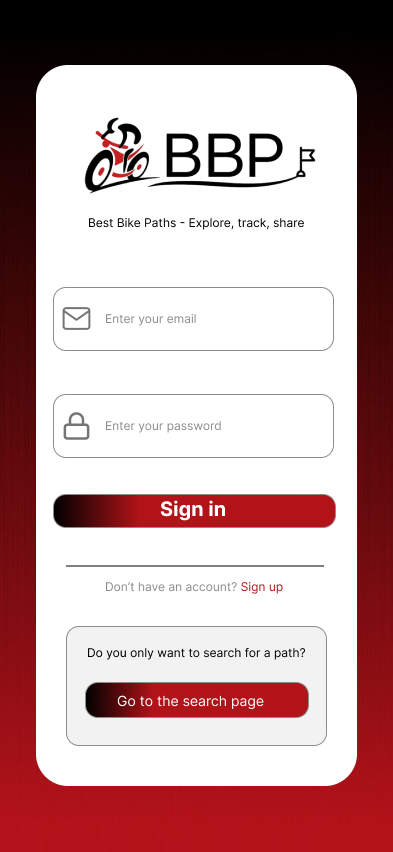
\includegraphics[width=\textwidth]{Images/User Interfaces/Sign in page.png}
    \caption{Sign in page of BBP.}
\end{minipage}
\hspace{1 cm}
\begin{minipage}{0.45\textwidth}
    \centering
    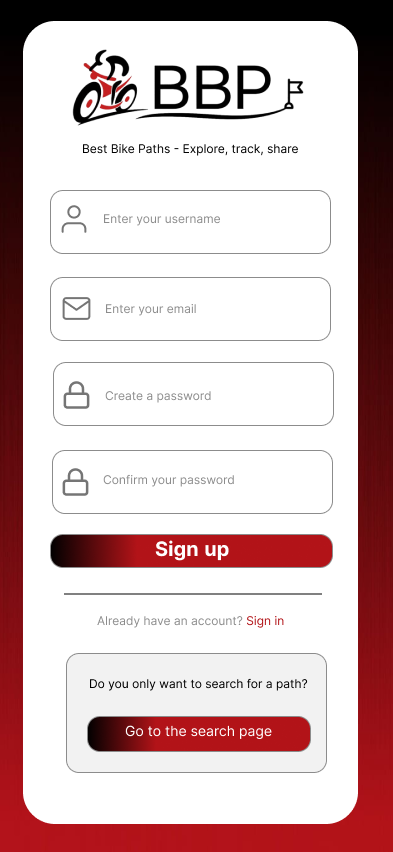
\includegraphics[width=\textwidth]{Images/User Interfaces/Sign up page.png}
     \caption{Sign up page of BBP.}
\end{minipage}

\end{figure}

\newpage

\begin{figure}[H]

\begin{minipage}[t]{0.45\textwidth}
    \vspace{0 pt}
    \framebox{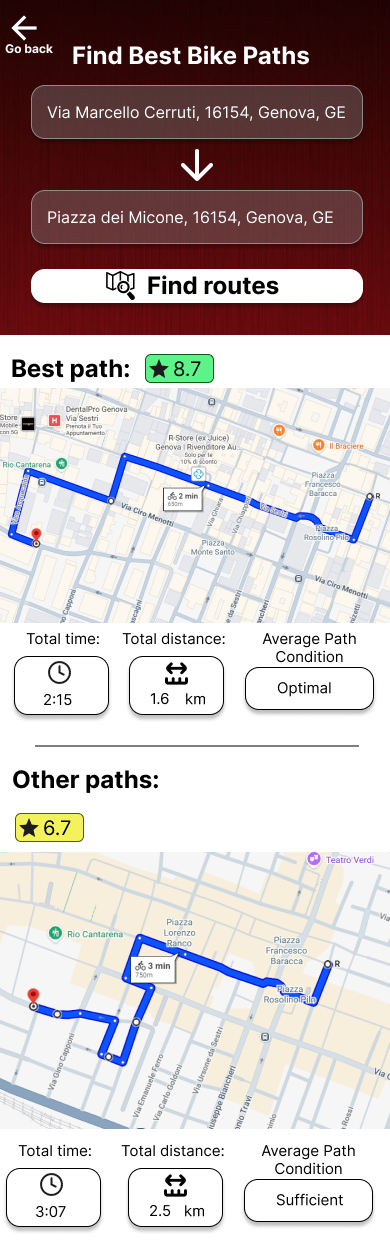
\includegraphics[width=\textwidth]{Images/User Interfaces/Find Best Bike Paths pt.1.png}}
\end{minipage}
\hspace{1 cm}
\begin{minipage}[t]{0.45\textwidth}
    \vspace{0 pt}
   \framebox{ 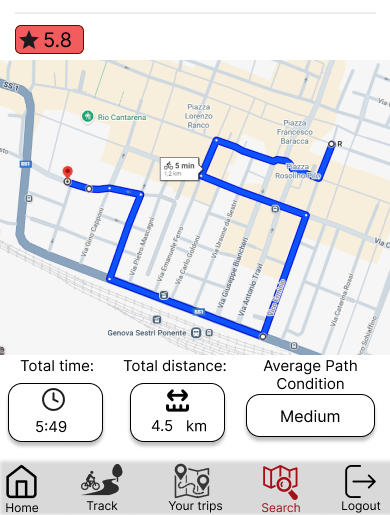
\includegraphics[width=\textwidth]{Images/User Interfaces/Find Best Bike Paths pt.2.png}}
     \caption{Possible screen visualization after a search in BBP. Note: If a User is not registered, the navigation bar is not present}
\end{minipage}

\end{figure}

\newpage

\textbf{User Interfaces for Registered Users only}

\begin{figure}[H]

\begin{minipage}{0.5\textwidth}
    \centering
    \framebox{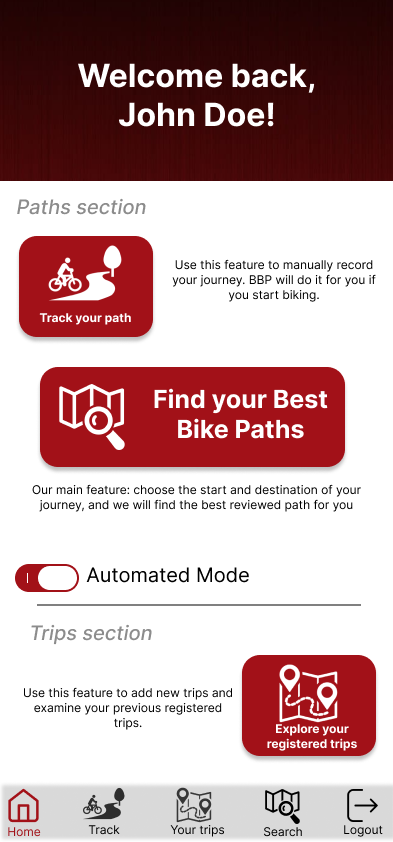
\includegraphics[width=\textwidth]{Images/User Interfaces/Home Page.png}}
    \caption{Home page of BBP.}
\end{minipage}
\hspace{1 cm}
\begin{minipage}{0.5\textwidth}
    \centering
    \framebox{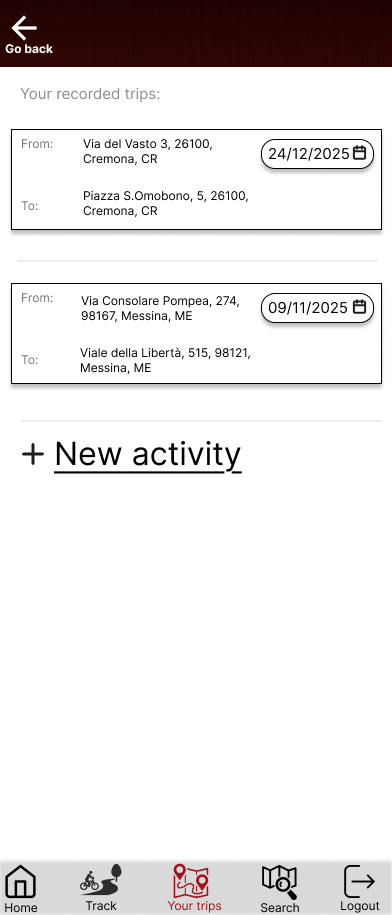
\includegraphics[width=\textwidth]{Images/User Interfaces/Seeing your trips.png}}
     \caption{List of trips registered (not published paths).}
\end{minipage}

\end{figure}

\newpage

\begin{figure}[H]

\begin{minipage}{0.45\textwidth}
    \centering
    \framebox{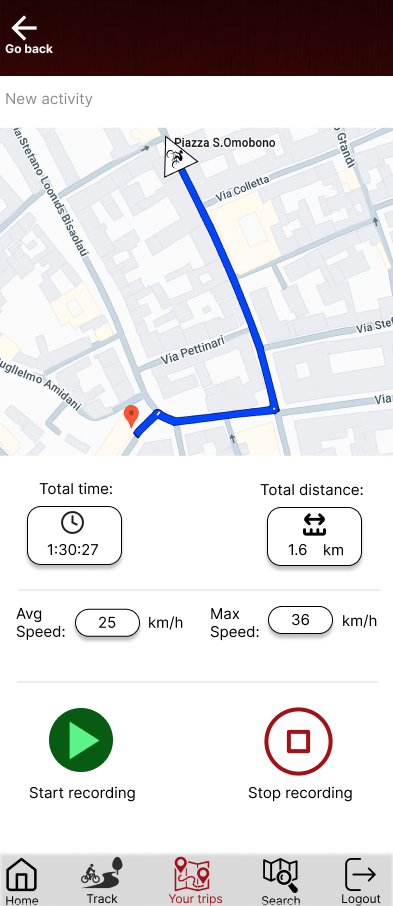
\includegraphics[width=\textwidth]{Images/User Interfaces/Adding new activity.png}}
    \caption{Recording a new activity using BBP.}
\end{minipage}
\hspace{1 cm}
\begin{minipage}{0.45\textwidth}
    \centering
    \framebox{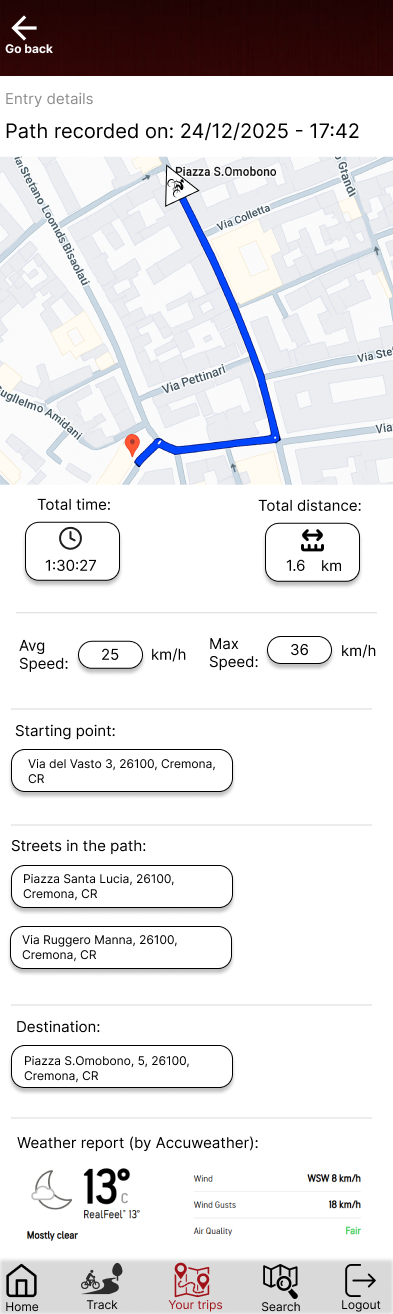
\includegraphics[width=\textwidth]{Images/User Interfaces/Entry details.png}}
     \caption{Reviewing your recorded activities using BBP.}
\end{minipage}
\end{figure}

\newpage

\begin{figure}[H]
\centering
\framebox{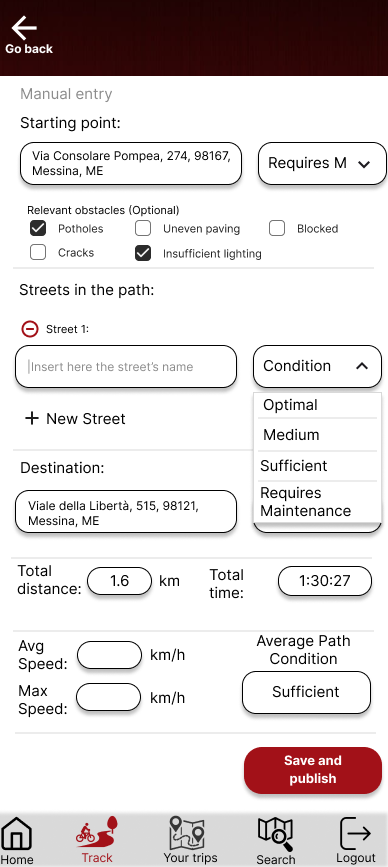
\includegraphics[width=0.5\textwidth]{Images/User Interfaces/Tracking page manual.png}}
\caption{Page used to insert tracked paths to be published and made available to every user.}
\end{figure}

\newpage

\begin{figure}[H]

\begin{minipage}{0.5\textwidth}
    \centering
    \framebox{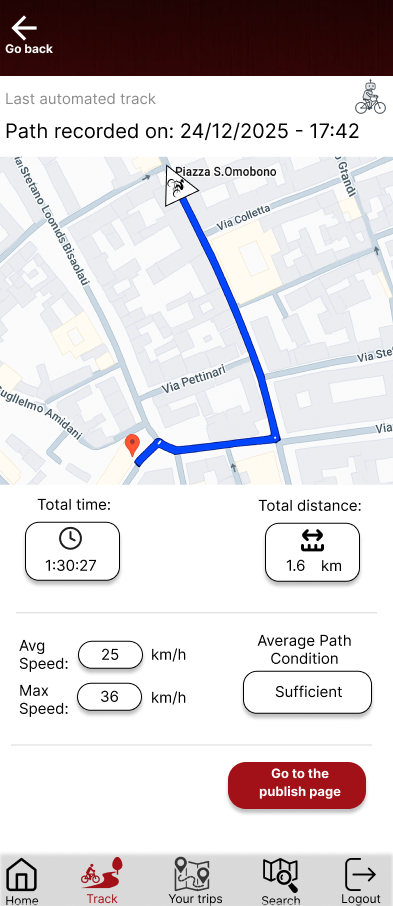
\includegraphics[width=\textwidth]{Images/User Interfaces/Tracking automated.png}}
    \caption{After doing an automated tracking of a path, this is the first screen the user sees when booting up the app.}
\end{minipage}
\hspace{1 cm}
\begin{minipage}{0.5\textwidth}
    \centering
    \framebox{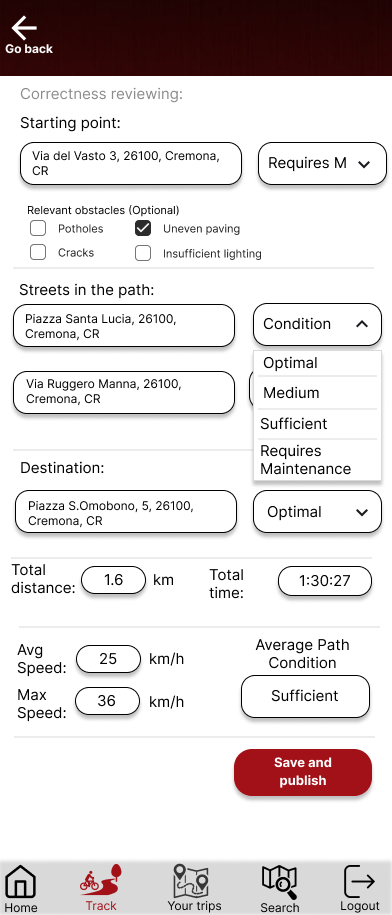
\includegraphics[width=\textwidth]{Images/User Interfaces/Tracking automated publish.png}}
     \caption{Reviewing the automated tracking paths before publishing them.}
\end{minipage}
\end{figure}

\subsubsection{Hardware Interfaces}

Our platform is a mobile application, requiring a portable device, such as a smartphone. Additional sensors are mandatory (either inside the device or connectable to be easily read by it):
\begin{itemize}
    \item \textbf{GPS}: used to gather reliable information regarding the biker's position in the map. It is needed to also accurately reconstruct the path performed by the user.
    \item \textbf{Gyroscope}: used to gather reliable information regarding the possible obstacles in the path (e.g. potholes).
    \item \textbf{Accelerometer}: used to gather reliable information regarding the possible obstacles in the path, the user's speed during the activity (maximum and average speed) and detect when the biker is starting or ending their activity (in automated mode).
\end{itemize}
A stable Internet connection is also required throughout the entirety of the recording, in particular during the saving of the recordings and the queries to search the best possible paths (both of these features require communication with the central server).

\subsubsection{Software Interfaces}
\subsubsection*{Email and Weather Report Systems}
In order to enrich the user experience, an external email delivery system ~\cite{aws_ses_2025} is used to send confirmation emails. Furthermore, trip data can be enriched by weather report systems ~\cite{OpenWeatherMapAPI}. To achieve this, the system relies on REST APIs as interfaces to the explained services and components.

\subsubsection*{Map rendering}
To make the user interface more accessible, a mapping SDK~\cite{MapsSDK} is used by BBP to show on-screen a map of the current location and the possible paths. The SDK provides APIs to draw tiles, overlays, pointers.

\subsubsection*{DBMS}
In order to store the entirety of the information that makes BPP work, a database and a management system is needed. Every DBMS provides APIs to perform actions to the data.

\subsubsection{Communication Interfaces}
Our system consists of two main parts: the mobile application and the backend system, that also communicate with several others components.

\subsubsection*{Communication between mobile application and system}
The mobile application must communicate with the backend system using the Internet protocols. This means that each interaction, in particular data transmission, must be secure and encrypted using REST APIs with HTTPS.
The purpose of this connection is in regard of the entirety of the user authentication process, the upload and the download of trip and path information.

\subsubsection*{Communication between mobile application and on-device sensors}
The mobile application must communicate with on-device sensors to retrieve data to be sent to the server, here stored, processed and made available to others. This communication happens through specific APIs for each and every sensor.

\subsubsection*{Communication between server and email provider}
The server must communicate with an email delivery system to send profile confirmation emails. For this purpose, REST APIs with HTTPS are still widely used. It is to note that the mobile application never communicates with the email provider system, all of the actions go through the server.

\subsubsection*{Communication between server and weather provider}
The server must communicate with an external weather providing system to send queries about current weather reports and receive data to attach to trip information. For this purpose, REST APIs with HTTPS are still widely used. It is to note that the mobile application never communicates with the weather report system, all of the actions go through the server.

\subsubsection*{Communication between server and database}
The server must communicate with a database system, to store and retrieve data about users, paths and trips. For this purpose, SQL queries are the basis of our communication.

\subsection{Functional Requirements}

\begin{enumerate}[label=•  R\arabic*:]

\subsubsection*{Sign up}

    \item The system must allow users to register using a username, an email and a password.
    \item The system must verify that credentials are unique.
    \item The system must send a verification email to the user.
    \item The system must let people verify their email after receiving the verification request.
    \item The system must activate accounts only if verified.

\subsubsection*{Login and Logout}
    \item The system must allow registered users to log in using email and password.
    \item The system must verify the correctness of the credentials.
    \item The system must allow registered users to log in only if the credentials are correct.
    \item The system must allow registered users, that logged-in, to log out.
    \item The system must delete user's session.
    \item The system must allow only registered users to record trips and submit new bike path information.
    \item The system must allow every user to access the system to browse paths.

\subsubsection*{Permissions}
    \item The system must ask registered users to give permissions for the sensors.
    \item The system must read the sensors data only if the permissions are given by the registered user.

\subsubsection*{Trip Management}

    \item The system must allow registered users to record their bike trips.
    \item The system must use sensors to track the biker's trip and their performance metrics.
    \item The system must allow the registered user to save the trip recorded.
    \item The system must check the availability of the Weather Reporting Service (WRS) before requesting data.
    \item The system must ask the WRS for weather information regarding the trip considered.
    \item The system must attach weather information to the trip entry, if available.
    \item The system must show registered users a list of their recorded trips.
    \item The system must allow registered users to see details of a specified recorded trip.

\subsubsection*{Bike Path Management - Manual mode}

    \item The system must allow registered users to manually insert path information using a form.
    \item The system must require the user to specify roads and intersections in the path.
    \item The system must allow registered users to specify the condition of each road in the path.
    \item The system must allow registered users to report additional issues (f.e. potholes).
    \item The system must save the path information in the central database.

\subsubsection*{Bike Path Management - Automated mode}
    \item The system must let registered users enable automated mode.
    \item The system must let registered users disable automated mode.
    \item The system must let registered users add path information via automated mode.
    \item The system must record data using sensors only if automated mode is enabled.
    \item The system must recognize if the registered user is biking.
    \item The system must start recording the path only if the system recognizes that the registered user is biking.
    \item The system must use the sensors' data to record the path.
    \item The system must record intersections and road crossed by the registered user.
    \item The system must recognize obstacles in the path (f.e. pothole) using sensors' data.
    \item The system must recognize if the registered user stopped biking.
    \item The system must stop recording the path if the system recognizes that the registered user stopped biking.
    \item The system must save the recorded bike path information in "to be reviewed" state after an automated mode recording
    \item The system must notify the user that a path has been recorded this way.
    \item The system must require registered users to review and edit information collected via automated mode before publishing.
    \item The system must allow registered users to discard the information collected via automated mode.
    \item The system must allow registered users to save and publish the information recorded via automated mode.
    

\subsubsection*{Finding the Best Path}
    \item The system must allow every user, regardless of their registration status, to browse for paths.
    \item The system must allow the user to fill up a form regarding an origin and destination point.
    \item The system must compute the best path(s) considering the specified points.
    \item The system must merge information from multiple users regarding a road, considering freshness of information and number of confirming users.
    \item The system must compute an average status for the specified path.
    \item The system must compute a score for the specified path, considering their status and the easy reachability.
    \item The system must show the user all the possible best paths in descendant score order, with their scores and metrics.
    \item The system must show the user a map of the best path(s).
\end{enumerate}

\subsubsection{Use Case Diagram ~\cite{UMLUseCaseDiagrams}} 
\begin{figure}[H]
\centering
\framebox{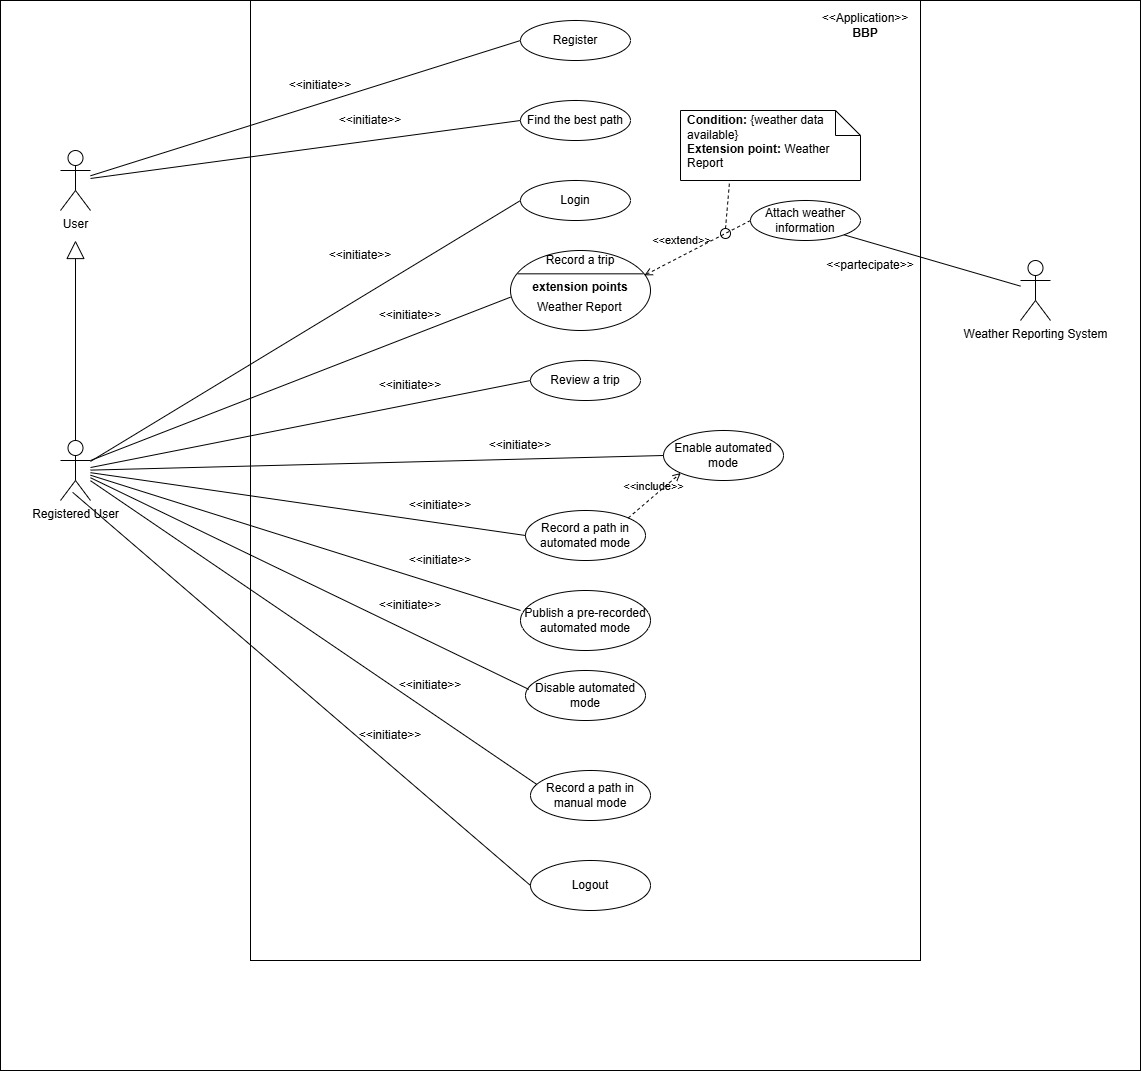
\includegraphics[width=\textwidth]{Images/Diagrams/Use Case/Use Case Diagram.jpg}}
\caption{Use Case Diagram}
\end{figure}
\newpage

\subsubsection{Use Cases}

\begin{enumerate}[label=\textbf{[UC\arabic*]}]

    \item \textbf{Register}
        \begin{center}
            \begin{tabular}{|p{4cm}|p{11cm}|}
                \hline
                \textbf{Name} & \textbf{Register} \\
                \hline
                Actors & User \\
                \hline
                Entry Condition & User opens the BBP platform \\
                \hline
                Event Flow & 
                1. The user presses "Don't have an account? Sign up" in the first page\\
                & 2. The system requires the user to fill out a form with the user's username, email address, and a password.\\
                & 3. The user inserts username, email address, and a password.\\
                & 4. The user presses the "Sign Up" button\\
                & 5. The system verifies that: \newline -the username does not exist yet \textbf{AND},\newline -the email address has not been registered yet. \\
                & 6. The system sends a verification email to the provided address.\\
                & 7. Outside the system, the user verifies the email address (provided in step 3) by clicking the link inside the email sent in step 6. \\
                \hline
                Exit Condition & The user has successfully registered to the platform \\
                \hline
                Exception & E1 - (6) The email cannot be delivered to the provided email address.\newline The system tries to send the email again and displays an error to the user if it fails again \\
                & E2 - (5) The username already exists.\newline In this case, the system displays an error to the user and asks them to try with another username. \\
                & E3 - (5) The email already exists.\newline In this case, the system display an error to the user and asks them to try with another email or if they want to login instead. \\
                \hline
            \end{tabular}
            \captionof{table}{Organization Registration Use Case}
        \end{center}
\newpage
    \item \textbf{Find the best path}
        \begin{center}
            \begin{tabular}{|p{4cm}|p{11cm}|}
                \hline
                \textbf{Name} & \textbf{Find the Best Path} \\
                \hline
                Actors & User \\
                \hline
                Entry Condition & One of the following conditions must hold: \newline -User opens the BBP platform \textbf{OR} \newline -User is in the home page\\
                \hline
                Event Flow & 1. The user initiates the route search by pressing one of the following buttons:\newline -"Go to the search page" \textbf{OR} \newline -"Find your Best Bike Paths" \textbf{OR} \newline -"Search" in the navigation bar. \\
                & 2. The system requires the user to insert an origin and a destination point. \\
                & 3. The user inserts the origin and destination point. \\
                & 4. The user presses the "Find routes" button.\\
                & 5. The system merges information from different users, considering freshness and number of confirming users.\\
                & 6. The system computes possible bike paths and their score between these points. \\
                & 7. The system displays paths and their scores in descendant score order. \\
                \hline
                Exit Condition & The user sees recommended bike paths with visualized scores and information about riding time, total distance and path condition. \\
                \hline
                Exception & E1 - (6) No valid path between selected points. \newline In this case, the system will provide the user with a blank page and a message saying that there not exists a path between those two points. \\
                & E2 - (6) System fails to retrieve path data.\newline In this case, the system tries again and, if not possible, warns the user to try again later. \\
                \hline
            \end{tabular}
            \captionof{table}{Find the best path Use Case}
        \end{center}
    
    \item \textbf{Login} 
        \begin{center}
            \begin{tabular}{|p{4cm}|p{11cm}|}
                \hline
                \textbf{Name} & \textbf{Login} \\
                \hline
                Actors & Registered User \\
                \hline
                Entry Condition & Registered user opens the platform \\
                \hline
                Event Flow & 1. The system prompts the registered user to enter email and password credentials. \\
                & 2. The registered user enters email and password credentials. \\
                & 3. The registered user presses the "Sign in" button. \\
                & 4. The system verifies validates entered credentials \\
                \hline
                Exit Condition & The registered user has successfully logged in to the platform \\
                \hline
                Exception & E1: (4) - Invalid credentials. \newline In this case, the system displays an error message "Invalid email or password" and prompts the registered user to try again.\\
                & E2: (4) - Email address not verified. \newline In this case, the system informs the registered user that the email has not been verified and prompts to try again.\\
                \hline
            \end{tabular}
            \captionof{table}{Login Use Case}
        \end{center}
\newpage
    \item \textbf{Record a Trip} 
        \begin{center}
            \begin{tabular}{|p{4cm}|p{11cm}|}
                \hline
                \textbf{Name} & \textbf{Record a trip} \\
                \hline
                Actors & Registered User \\
                \hline
                Entry Condition & Registered user is logged in \\
                \hline
                Event Flow & 1. The registered user goes to the registered trips section by: \newline -pressing the "Track your path" button \textbf{OR},\newline -pressing the "Your Trips" button in the navigation bar.\\
                & 2. The registered user presses the "New Activity" button. \\
                & 3. The system displays the “New Activity” page, prompting the user to start recording.\\
                & 4. The registered user presses the "Start recording" button. \\
                & 5. The system starts recording the trip, collecting GPS location, speed, and sensor data. \\
                & 6. The registered user can pause or resume the recording. \\
                & 7. The registered user stops the recording. \\
                & 8. The system saves the trip information and displays a summary including total time, average speed, and total distance. \\
                \hline
                Exit Condition & Trip is stored with performance metrics \\
                \hline
                Exception & E1: (5) - GPS/sensor data not available\newline In this case, the system displays an error to the registered user, describing the problem and suggesting to check the sensors or try again another time. \\
                & E2: (8) Error saving the data into the system\newline In this case, the system tries to save again until it is successfully saved. \\
                & E3: (5) The application crashes during the recording\newline In this case, the system pauses the recording and, at the reboot of the application, prompts the registered user to save it or start it again. \\
                & E4: (4) Permissions not granted\newline The system prompts the registered user for access to the sensors and background execution. If the registered user denies permissions, the system disables automated mode and notifies the registered user.\\
                \hline
                Extension Point: & Step 8 - Optional: Trigger Weather Report\\
                \hline
            \end{tabular}
            \captionof{table}{Record a trip Use Case}
        \end{center} 

    \item \textbf{Attach weather information} 
        \begin{center}
            \begin{tabular}{|p{4cm}|p{11cm}|}
                \hline
                \textbf{Name} & \textbf{Attach weather information} \\
                \hline
                Actors & Weather Reporting System (WRS) \\
                \hline
                Entry Condition & A trip without weather data is recorded \\
                \hline
                Event Flow & 1. The system checks the availability of the Weather Reporting System (WRS). \\
                & 2. The WRS responds with its availability. \\
                & 3. The system requests contextual weather data for the trip from the WRS. \\
                & 4. The WRS provides meteorological information, including wind speed, temperature, and weather conditions. \\
                & 5. The system attaches the received weather information to the trip record. \\
                \hline
                Exit Condition & Trip is stored with performance metrics and weather information \\
                \hline
                Exception & E1 - (1) WRS not available.\newline In this case, the system acts like no weather information were available and does not attach anything to the trip. \\
                & E2 - (3) Weather data not available.\newline In this case, the system does not attach anything to the trip information.\\
                \hline
            \end{tabular}
            \captionof{table}{Attach weather information Use Case}
        \end{center}
\newpage
    \item \textbf{Review a trip} 
        \begin{center}
            \begin{tabular}{|p{4cm}|p{11cm}|}
                \hline
                \textbf{Name} & \textbf{Review a Trip} \\
                \hline
                Actors & Registered User \\
                \hline
                Entry Condition & Registered user is logged in \\
                \hline
                Event Flow & 1. The registered user goes to the registered trips section by: \newline -pressing the "Explore your registered trips" button \textbf{OR},\newline -pressing the "Your Trips" button in the navigation bar.\\
                & 2. The system displays a list of recorded trips, showing the starting and finishing points, and the date of each trip. \\
                & 3. The registered user presses on a trip. \\
                & 4. The system displays a detailed view with the information of the selected trip, including all recorded information.. \\
                \hline
                Exit Condition & The registered user reviews trip data. \\
                \hline
                Exception & E1 - No registered trip associated with the registered user. \newline In this case, the system shows an empty page to the registered user.\\
                 & E2 - Error fetching trip information \newline In this case, the system displays an error message to the registered user, inviting to try again later.\\
                \hline
            \end{tabular}
            \captionof{table}{Review a trip Use Case} 
        \end{center} 


    \item \textbf{Record a Path in Automated Mode}
            \begin{center}
                \begin{tabular}{|p{4cm}|p{11cm}|}
                    \hline
                    \textbf{Name} & \textbf{Record a Path in Automated Mode} \\
                    \hline
                    Actors & Registered User \\
                    \hline
                    Entry Condition & All of these conditions must hold: \newline -Registered user is logged in \textbf{AND}, \newline -Automated mode is enabled.\\
                    \hline
                    Event Flow & 1. The registered user begins a bike ride with automated mode already enabled -> see ~\hyperref[EAM]{Enable Automated Mode} \\
                    & 2. The system records GPS, accelerometer, and gyroscope data while the user is cycling. \\
                    & 3. The system detects possible obstacles or potholes from sensor data and saves the information. \\
                    & 4. The registered user stops biking. \\
                    & 5. The system detects when the user ended the bike ride. \\
                    & 6. The system saves the recorded bike path information \\
                    & 7. The system notifies the registered user that a new path has been recorded. \\
                    \hline
                    Exit Condition & Path information is stored and is ready for review. \\
                    \hline
                    Exception & E1: (2) - GPS/sensor data not available\newline In this case, the system displays an error to the registered user, describing the problem and suggesting to check the sensors or try again another time. \\
                    & E2: (6) Error saving the data into the system\newline In this case, the system tries to save again until it is successfully saved. \\
                    & E3: (2) The application crashes during the recording\newline In this case, the system stops the recording and, at the reboot of the application, acts as if the recording has ended normally. \\
                    \hline
                \end{tabular}
                \captionof{table}{Record a Path in Automated Mode Use Case}
            \end{center}
\newpage
    \item \textbf{Enable Automated Mode}
        \label{EAM}
        \begin{center}
            \begin{tabular}{|p{4cm}|p{11cm}|}
                \hline
                \textbf{Name} & \textbf{Enable Automated Mode} \\
                \hline
                Actors & Registered User \\
                \hline
                Entry Condition & Registered user is logged in \\
                \hline
                Event Flow & 1. The registered user presses the toggle button "Automated mode" \\
                & 2. The system starts collecting data from the device's sensors (GPS, accelerometer, gyroscope) \\
                & 3. The system notifies the registered user that automatic mode is enabled. \\
                \hline
                Exit Condition & The system actively collects bike path and sensor data \\
                \hline
                Exception & E1: (1) Permissions not granted\newline The system prompts the user for access to the sensors and background execution. If the user denies permissions, the system disables automated mode and notifies the user. \\
                &  E2: (2) - GPS/sensor error\newline In this case, the system displays an error to the user, describing the problem and suggesting to check the sensors or try again another time. \\
                \hline
            \end{tabular}
            \captionof{table}{Enable Automated Mode Use Case}
        \end{center}

    \item \textbf{Disable Automated Mode}
        \begin{center}
            \begin{tabular}{|p{4cm}|p{11cm}|}
                \hline
                \textbf{Name} & \textbf{Disable Automated Mode} \\
                \hline
                Actors & Registered User \\
                \hline
                Entry Condition & All of these conditions must hold: \newline -Registered user is logged in \textbf{AND}, \newline -Automated mode is enabled.\\
                \hline
                Event Flow & 1. The registered user presses the toggle button "Automated mode" \\
                & 2. The system stops collecting data from the device's sensors (GPS, accelerometer, gyroscope) \\
                & 3. The system notifies the registered user that automatic mode is disabled. \\
                \hline
                Exit Condition & System is no longer collecting bike path and sensor data \\
                \hline
                Exception & E1: (1) Trip/Path recording in progress \newline 
                In this case, the system stops recording the trip/path. \\
                &  E2: (2) - GPS/sensor error\newline In this case, the system displays an error to the registered user, describing the problem and suggesting to check the sensors or try again another time. \\
                \hline
            \end{tabular}
            \captionof{table}{Disable Automated Mode Use Case}
        \end{center}
\newpage
        \item \textbf{Publish a pre-recorded automated mode path}
        \begin{center}
            \begin{tabular}{|p{4cm}|p{11cm}|}
                \hline
                \textbf{Name} & \textbf{Publish a pre-recorded automated mode path} \\
                \hline
                Actors & Registered User \\
                \hline
                Entry Condition & Registered user is logged in, automated mode is enabled, and a path has been recorded \\
                \hline
                Event Flow & 1. The system notifies the registered user that a new path has been recorded and is ready to be reviewed. \\
                & 2. The user accesses the recorded path by either pressing the notification \textbf{OR} opening the application after ending the recording. \\
                & 3. The system displays the recorded path information \\
                & 4. The system prompts the registered user to either confirm, edit, or delete the recorded path information.\\
                & 5. The registered user reviews and, if necessary, edits the path information. \\
                & 6. The registered user presses "Save and publish". \\
                & 7. The system saves the path information in the central database, making it available for other users. \\
                \hline
                Exit Condition & Path information is stored and is published \\
                \hline
                Exception & E1: (4) The registered user deletes the recording.\newline In this case, the recording is discarded.\\
                & E2: (7) Error saving the data into the system\newline In this case, the system tries to save again until it is successfully saved. \\
                \hline
            \end{tabular}
            \captionof{table}{Publish a pre-recorded automated mode path Use Case}
        \end{center}

    \item \textbf{Record a Path in Manual Mode}
        \begin{center}
            \begin{tabular}{|p{4cm}|p{11cm}|}
                \hline
                \textbf{Name} & \textbf{Record a Path in Manual Mode} \\
                \hline
                Actors & Registered User \\
                \hline
                Entry Condition & Registered user is logged in \\
                \hline
                Event Flow & 1. The registered user goes to the registered trips section by: \newline -pressing the "Track your path" button \textbf{OR},\newline -pressing the "Track" button in the navigation bar.\\
                & 2. The system prompts the registered user to provide path information via a form. \\
                & 3. The registered user fills out the form with the streets and intersections forming the path, specifying the status of each road and detailing any issues if the road is not optimal.\\
                & 4. The registered user presses "Save and publish" \\
                & 5. The system saves the path information in the central database, making it publicly available for other users. \\
                \hline
                Exit Condition & Path information is stored and can be made publishable \\
                \hline
                Exception & E1: (3) Mandatory data not provided \newline In this case, the system displays a message to the registered user, prompting them to add the missing details. \\
                & E2: (7) Error saving the data into the system\newline In this case, the system tries to save again until it is not saved. \\
                & E3: (4) The registered user deletes the entry\newline In this case, the system discards the path. \\
                \hline
            \end{tabular}
            \captionof{table}{Record a path in manual mode Use Case}
        \end{center}
\newpage
        \item \textbf{Logout}
        \begin{center}
            \begin{tabular}{|p{4cm}|p{11cm}|}
                \hline
                \textbf{Name} & \textbf{Logout} \\
                \hline
                Actors & Registered User \\
                \hline
                Entry Condition & Registered user is logged in. \\
                \hline
                Event Flow & 1. Registered user presses "Logout" on the navigation bar. \\
                & 2. The system prompts the registered user to confirm the logout action. \\
                & 3. The registered user confirms. \\
                & 4. The system revokes the user’s session credentials and clears all session-related data.\\
                & 5. The system redirects the user to the login page. \\
                \hline
                Exit Condition & Registered user is no longer authenticated; session is closed \\
                \hline
                Exception & E1: (4) Error to terminate session correctly. \newline In this case, the system retries to terminate session correctly until it is possible.\\
                & E2: (2) The registered user cancels the logout action.\newline In this case, the system redirects the registered user to the home page.\\
                \hline
            \end{tabular}
            \captionof{table}{Logout Use Case}
        \end{center}
    
\end{enumerate}
\subsubsection{Mapping}

\begin{table}[H]
\begin{tabular}{|p{5cm}|p{5cm}|p{5cm}|}
\hline
\textbf{Goal} & \textbf{Requirements and Domain\newline Assumptions} & \textbf{Use cases}\\
\hline
\textbf{G1}: Users can register and have a profile in BBP application. & \begin{tabular}[c]{@{}p{5cm}@{}} \textbf{R1}: The system must allow users to register using a username, an email and a password.\\ \hline \textbf{R2}: The system must verify that credentials are unique. \\ \hline \textbf{R3}: The system must send a verification email to the user. \\ \hline \textbf{R4}: The system must let people verify their email after receiving the verification request. \\ \hline \textbf{R5}: The system must activate accounts only if verified. \\ \hline \textbf{R6}: The system must allow registered users to log in using email and password.\\ \hline \textbf{R7}: The system must verify the correctness of the credentials.\\ \hline \textbf{R8}: The system must allow registered users to log in only if the credentials are correct. \\ \hline \textbf{R9}: The system must allow registered users, that logged-in, to log out. \\ \hline \textbf{R10}: The system must delete user’s session.\\ \hline \hline \textbf{D2}: The internet connection remains relatively stable throughout the session. \\ \hline \textbf{D13}: Users will give non-misleading information about their identity. \end{tabular} & \begin{tabular}[c]{@{}p{5cm}@{}}\textbf{UC1}: Register\\ \hline \textbf{UC3}: Login \\ \hline \textbf{UC12}: Logout\end{tabular}\\
\hline
\end{tabular}
\end{table}


\begin{table}[H]
\begin{tabular}{|p{5cm}|p{5cm}|p{5cm}|}
\hline
\textbf{Goal} & \textbf{Requirements and Domain\newline Assumptions} & \textbf{Use cases}\\
\hline
\textbf{G2}: Users manually create bike paths in an inventory by specifying the name of the streets and the status. & \begin{tabular}[c]{@{}p{5cm}@{}} \textbf{R23}: The system must allow registered users to manually insert path information using a form.\\ \hline \textbf{R24}: The system must require the user to specify roads and intersections in the path. \\ \hline \textbf{R25}: The system must allow registered users to specify the condition of each road in the path. \\ \hline \textbf{R26}: The system must allow registered users to report additional issues (f.e. potholes). \\ \hline \textbf{R27}: The system must save the path information in the central database. \\  \hline \hline \textbf{D2}: The internet connection remains relatively stable throughout the session. \\ \hline \textbf{D4}: Users are expected to provide accurate and non-misleading information when creating new paths. \\ \hline \textbf{D5}: Users do not use the application or the platform for purposes unrelated to biking activities or the exploration of new routes as a recreational activity. \\ \hline \textbf{D8}: The date related to the new inserted path is correct. \\ \hline \textbf{D9}: The app is used where bike track already exists. \\ \hline \textbf{D10}: The biking paths have little to no cars presence. \\ \hline \textbf{D11}: The biking paths have speed limits compatible with the average speed of a bike.  \end{tabular} & \begin{tabular}[c]{@{}p{5cm}@{}}\textbf{UC11}: Record a path in manual mode\end{tabular}\\
\hline
\end{tabular}
\end{table}

%-----GOAL 3 TABLES (divided in two because of space-----%
\begin{table}[H]
\begin{tabular}{|p{5cm}|p{5cm}|p{5cm}|}
\hline
\textbf{Goal} & \textbf{Requirements and Domain\newline Assumptions} & \textbf{Use cases}\\
\hline
\textbf{G3}:Users create bike paths in an automated mode where the system acquire data from the user’s mobile device and reconstruct the path. & \begin{tabular}[c]{@{}p{5cm}@{}} \textbf{R13}: The system must ask registered users to give permissions for the sensors.\\ \hline \textbf{R14}: The system must read the sensors data only if the permissions are given by the registered user. \\ \hline \textbf{R28}: The system must let registered users enable automated mode.\\ \hline \textbf{R29}: The system must let registered users disable automated mode. \\ \hline \textbf{R30}: The system must let registered users add path information via automated mode.\\ \hline \textbf{R31}: The system must record data using sensors only if automated mode is enabled. \\ \hline \textbf{R32}:The system must recognize if the registered user is biking.\\ \hline \textbf{R33}: The system must start recording the path only if the system recognizes that the registered user is biking. \\ \hline \textbf{R34}: The system must use the sensors’ data to record the path.\\ \hline \textbf{R35}: The system must record intersections and road crossed by the registered user. \\ \hline \textbf{R36}:The system must recognize obstacles in the path (f.e. pothole) using sensors’ data.\\ \hline \textbf{R37}: The system must recognize if the registered user stopped biking. \\ \hline \textbf{R38}:The system must stop recording the path if the system recognizes that the registered user stopped biking.\\ \hline \textbf{R39}: The system must save the recorded bike path information in "to be reviewed" state after an automated mode recording \\ \hline \textbf{R40}: The system must notify the user that a path has been recorded this way.\\ \hline \textbf{R41}: The system must require registered users to review and edit information collected via automated mode before publishing. \\ \hline \textbf{R42}: The system must allow registered users to discard the information collected via automated mode.\\ \hline \textbf{R43}: he system must allow registered users to save and publish the information recorded via automated mode.\end{tabular} & \begin{tabular}[c]{@{}p{5cm}@{}}\textbf{UC6}: Enable automated mode \\ \hline \textbf{UC7}: Record a path in automated mode. \\ \hline \textbf{UC8}: Publish a pre-recorded automated mode path. \\ \hline \textbf{UC9}: Disable automated mode.  \end{tabular}\\

\end{tabular}
\end{table}

\begin{table}[H]
\begin{tabular}{|p{5cm}|p{5cm}|p{5cm}|}
 & \begin{tabular}[c]{@{}p{5cm}@{}} \textbf{R27}: The system must save the path information in the central database.\\ \hline \hline  \textbf{D1}: Each user rides a bicycle while the application runs in background in case of automated mode. \\ \hline \textbf{D2}: The internet connection remains relatively stable throughout the session. \\ \hline \textbf{D3}: Users are willing to review and refine the automatically collected information gathered by the device in
the automated-mode. \\ \hline \textbf{D4}: Users are expected to provide accurate and non-misleading information when creating new paths. \\ \hline \textbf{D5}: Users do not use the application or the platform for purposes unrelated to biking activities or the exploration of new routes as a recreational activity. \\ \hline \textbf{D6}: Third-parties services provide reliable information to the application.\\ \hline \textbf{D7}: Hardware devices must provide reliable sensor data to the system to let it acquire the right performance data. \\ \hline \textbf{D8}: The date related to the new inserted path is correct. \\ \hline \textbf{D9}: The app is used where bike track already exists. \\ \hline \textbf{D10}: The biking paths have little to no cars presence. \\ \hline \textbf{D11}: The biking paths have speed limits compatible with the average speed of a bike. \\ \hline \textbf{D12}: Users will stop cycling when they want to end the recording of the path. \end{tabular} & \\
\hline
\end{tabular}
\end{table}
\newpage


\begin{table}[H]
\begin{tabular}{|p{5cm}|p{5cm}|p{5cm}|}
\hline
\textbf{Goal} & \textbf{Requirements and Domain\newline Assumptions} & \textbf{Use cases}\\
\hline
\textbf{G4}: Users browse bike paths within the inventory. They can specify an origin and destination and ask the system to visualize the bike path on a map. & \begin{tabular}[c]{@{}p{5cm}@{}} \textbf{R44}: The system must allow every user, regardless of their registration status, to browse for paths.\\ \hline \textbf{R45}: The system must allow the user to fill up a form regarding an origin and destination point. \\ \hline \textbf{R46}: The system must compute the best path(s) considering the specified points. \\ \hline \textbf{R50}: The system must show the user all the possible best paths in descendant score order, with their scores and metrics. \\ \hline \textbf{R51}: The system must show the user a map of the best path(s). \\  \hline \hline \textbf{D2}: The internet connection remains relatively stable throughout the session. \end{tabular} & \begin{tabular}[c]{@{}p{5cm}@{}}\textbf{UC2}: Find the best path.\end{tabular}\\  
\hline
\end{tabular}
\end{table}

\begin{table}[H]
\begin{tabular}{|p{5cm}|p{5cm}|p{5cm}|}
\hline
\textbf{Goal} & \textbf{Requirements and Domain\newline Assumptions} & \textbf{Use cases}\\
\hline
\textbf{G5}: Users record their trips and store them to keep track of their cycling activities.    & \begin{tabular}[c]{@{}p{5cm}@{}} \textbf{R13}: The system must ask registered users to give permissions for the sensors.\\ \hline \textbf{R14}: The system must read the sensors data only if the permissions are given by the registered user. \\ \hline \textbf{R15}: The system must allow registered users to record their bike trips. \\ \hline \textbf{R16}: The system must use sensors to track the biker’s trip and their performance metrics. \\ \hline \textbf{R17}: The system must allow the registered user to save the trip recorded. \\  \hline \hline \textbf{D2}: The internet connection remains relatively stable throughout the session. \\ \hline \textbf{D5}: Users do not use the application or the platform for purposes unrelated to biking activities or the exploration of new routes as a recreational activity. \\ \hline \textbf{D7}:  Hardware devices must provide reliable sensor data to the system to let it acquire the right performance
data. \\ \hline \textbf{D8}: The date related to the new inserted path is correct. \\ \hline \textbf{D9}: The app is used where bike track already exists. \\ \hline \textbf{D10}: The biking paths have little to no cars presence. \\ \hline \textbf{D11}: The biking paths have speed limits compatible with the average speed of a bike.  \end{tabular} & \begin{tabular}[c]{@{}p{5cm}@{}}\textbf{UC4}: Record a trip. \end{tabular}\\
\hline
\end{tabular}
\end{table}

\begin{table}[H]
\begin{tabular}{|p{5cm}|p{5cm}|p{5cm}|}
\hline
\textbf{Goal} & \textbf{Requirements and Domain\newline Assumptions} & \textbf{Use cases}\\
\hline
\textbf{G6}: Users can see for a recorded trip various statistical data of the user performances as well as meteorological information during the respective trip.  & \begin{tabular}[c]{@{}p{5cm}@{}} \textbf{R18}: The system must check the availability of the Weather Reporting Service (WRS) before requesting data.\\ \hline \textbf{R19}: The system must ask the WRS for weather information regarding the trip considered. \\ \hline \textbf{R20}: The system must attach weather information to the trip entry, if available. \\ \hline \textbf{R21}: The system must show registered users a list of their recorded trips. \\ \hline \textbf{R22}: The system must allow registered users to see details of a specified recorded trip. \\  \hline \hline  \textbf{D6}: Third-parties services provide reliable information to the application. \\ \hline \textbf{D8}: The date related to the new inserted path is correct.  \end{tabular} & \begin{tabular}[c]{@{}p{5cm}@{}}\textbf{UC5}: Attach weather information. \\ \hline \textbf{UC6}: Review a trip.\\ \hline \end{tabular}\\
\hline
\end{tabular}
\end{table}

\begin{table}[H]
\begin{tabular}{|p{5cm}|p{5cm}|p{5cm}|}
\hline
\textbf{Goal} & \textbf{Requirements and Domain\newline Assumptions} & \textbf{Use cases}\\
\hline
\textbf{G7}: The system uses information published by the users about the paths by merging pieces of information to
generate the optimal path, using the freshness and number of confirmed data.  & \begin{tabular}[c]{@{}p{5cm}@{}} \textbf{R47}: The system must merge information from multiple users regarding a road, considering freshness of information and number of confirming users.\\ \hline \textbf{R48}: The system must compute an average status for the specified path. \\ \hline \textbf{R49}: The system must compute a score for the specified path, considering their status and the easy reachability. \\  \hline \hline \textbf{D2}: The internet connection remains relatively stable throughout the session.\\ \hline \textbf{D4}: Users are expected to provide accurate and non-misleading information when creating new paths.\\ \hline \textbf{D8}: The date related to the new inserted path is correct. \end{tabular} & \begin{tabular}[c]{@{}p{5cm}@{}}\textbf{UC2}: Find the best path.\end{tabular}\\  
\hline
\end{tabular}
\end{table}

\subsubsection{Sequence Diagrams ~\cite{UMLSequenceDiagrams}}

This subsection presents notifications modeled at a high level to illustrate user interactions. It deliberately omits detailed design, architectural considerations, and synchronization aspects to focus on the conceptual interaction flow rather than implementation specifics.

\begin{enumerate}[label=\textbf{[UC\arabic*]}]

\pagebreak
\item \textbf{Register}
\begin{figure}[H]
\centering
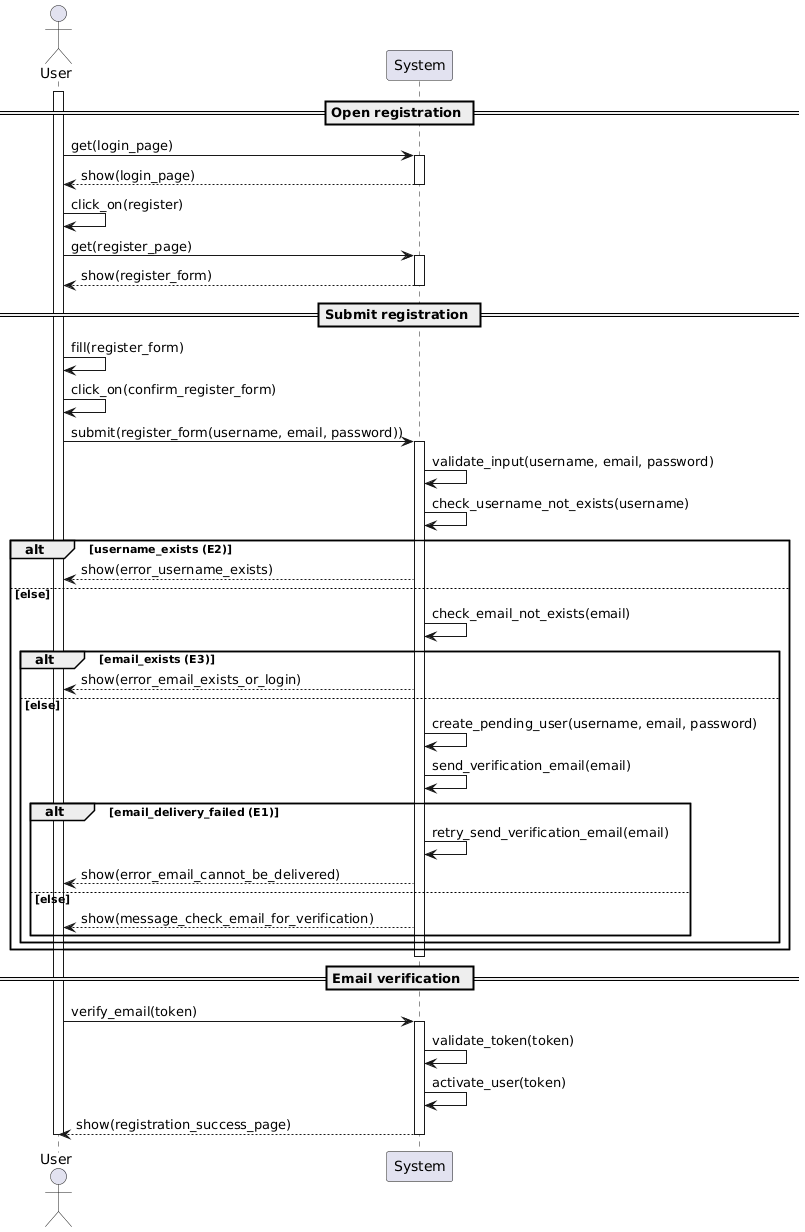
\includegraphics[scale=0.51]{RASD/Images/Diagrams/Sequence/register_sequence.png}
\caption{\label{fig:squencediagram}Sequence diagram for register.}
\end{figure}

\item \textbf{Find the best path}

\begin{figure}[H]
\centering
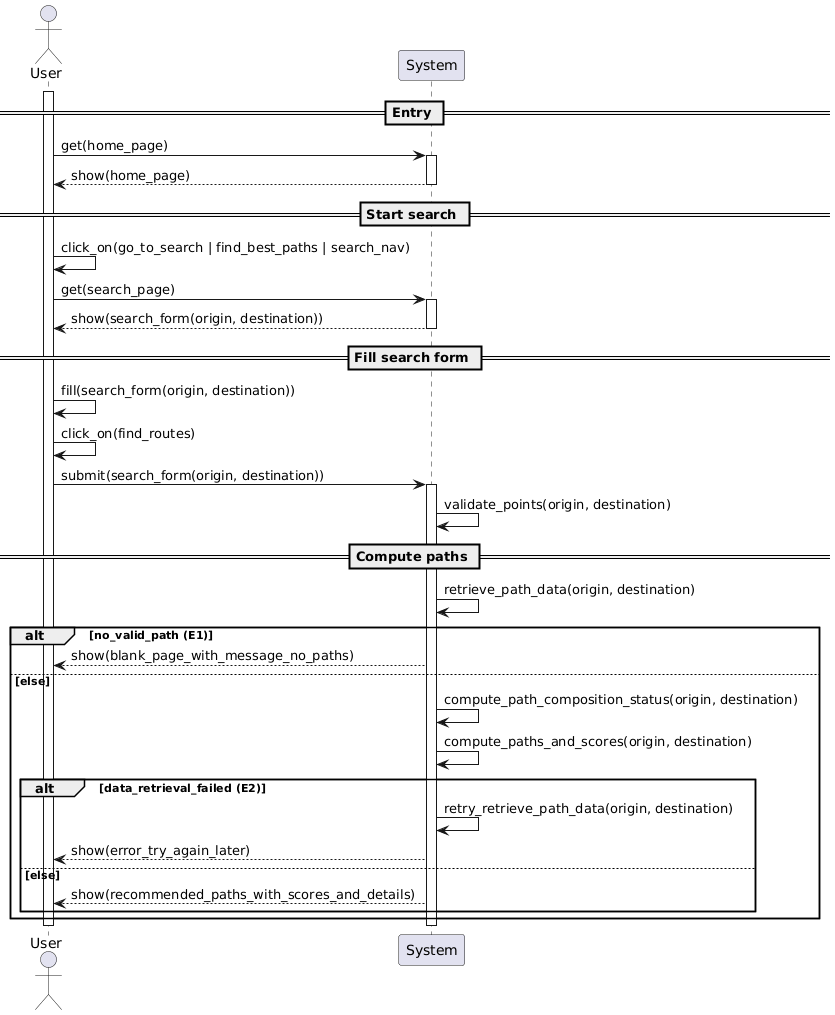
\includegraphics[width=\textwidth]{Images/Diagrams/Sequence/find_best_paths.png}
\caption{\label{fig:squencediagram}Sequence diagram for find best path.}
\end{figure}

\pagebreak

\item \textbf{Login}

\begin{figure}[H]
\centering
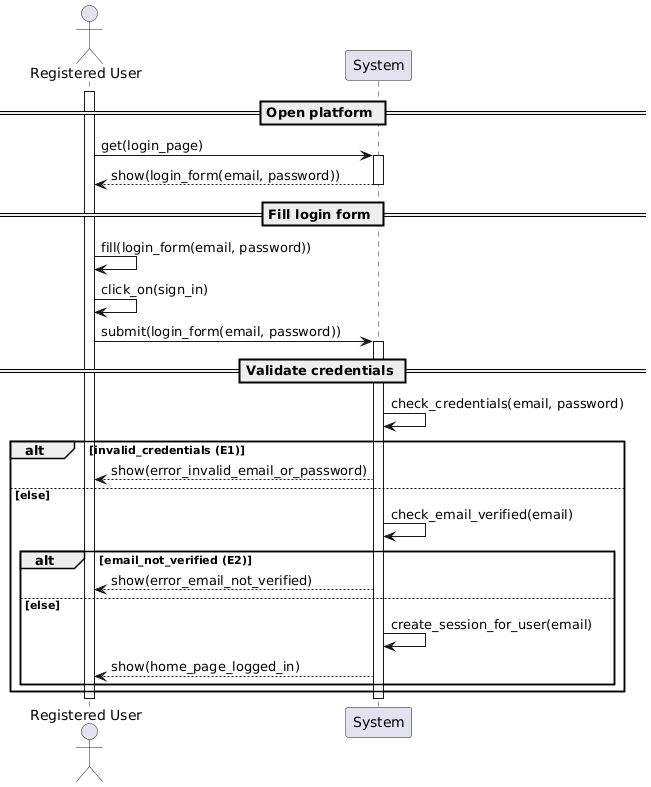
\includegraphics[width=\textwidth]{Images/Diagrams/Sequence/login.png}
\caption{\label{fig:squencediagram}Sequence diagram for login.}
\end{figure}

\pagebreak

\item \textbf{Record a Trip}

\begin{figure}[H]
\centering
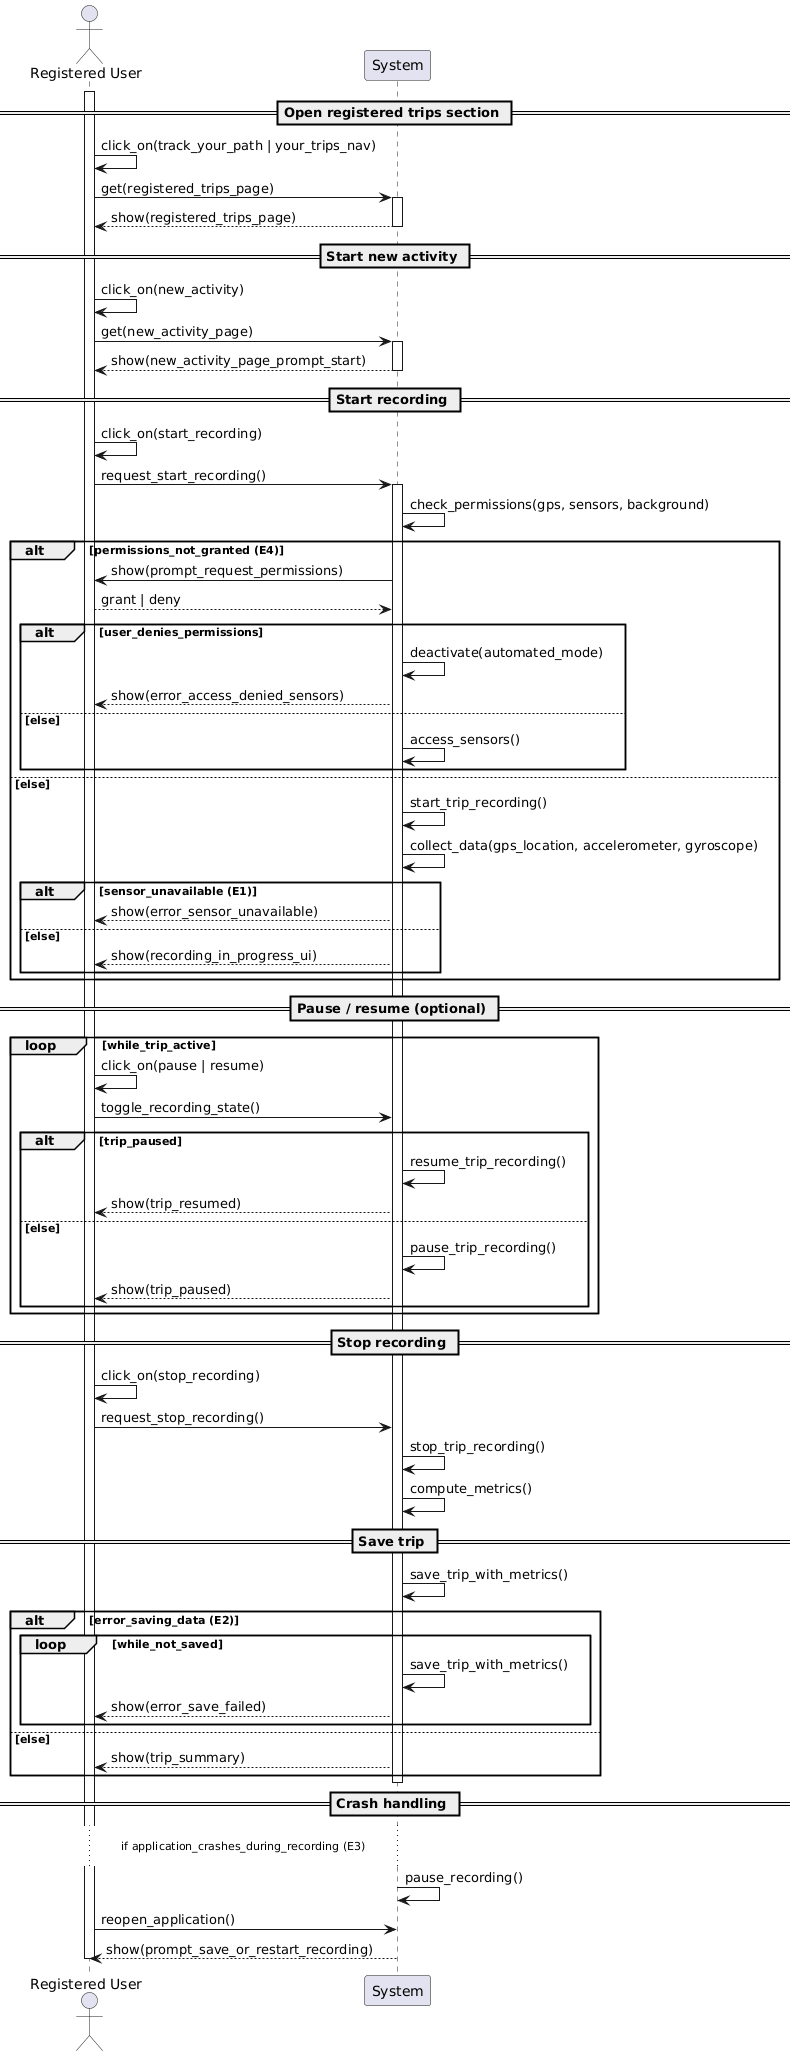
\includegraphics[scale=0.3]{Images/Diagrams/Sequence/record_trip.png}
\caption{\label{fig:squencediagram}Sequence diagram for record trip.}
\end{figure}

\pagebreak

\item \textbf{Attach weather information}

\begin{figure}[H]
\centering
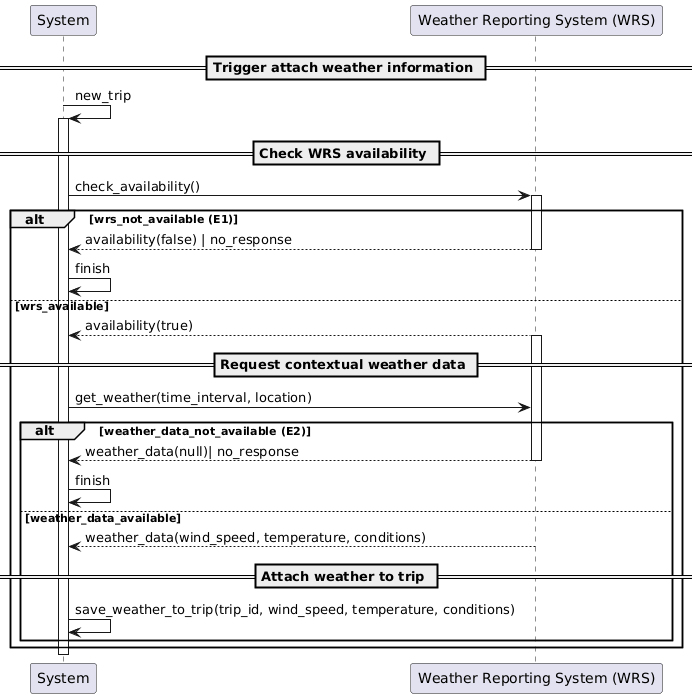
\includegraphics[width=\textwidth]{Images/Diagrams/Sequence/attach_weather.png}
\caption{\label{fig:squencediagram}Sequence diagram for attach weather information.}
\end{figure}

\pagebreak

\item \textbf{Review a trip}

\begin{figure}[H]
\centering
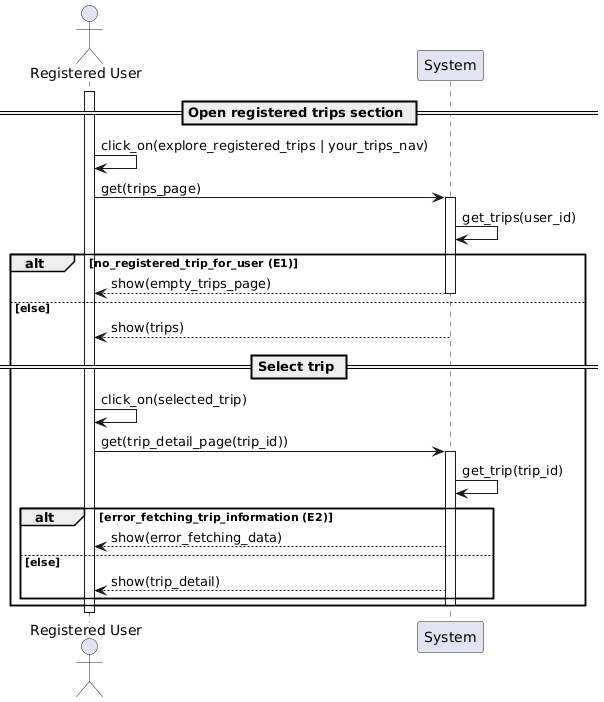
\includegraphics[width=\textwidth]{Images/Diagrams/Sequence/review_trip.png}
\caption{\label{fig:squencediagram}Sequence diagram for review trip.}
\end{figure}

\pagebreak

\item \textbf{Enable Automated Mode}

\begin{figure}[H]
\centering
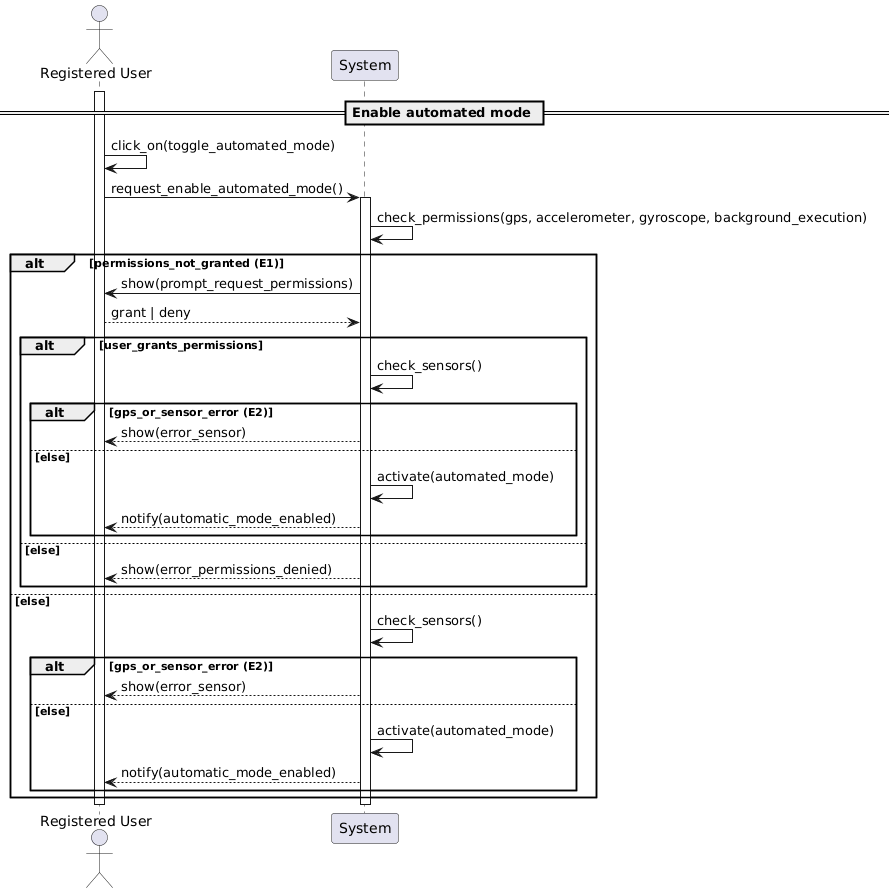
\includegraphics[width=\textwidth]{Images/Diagrams/Sequence/enable_auto_mode.png}
\caption{\label{fig:squencediagram}Sequence diagram for enable automated mode.}
\end{figure}

\pagebreak

\item \textbf{Disable Automated Mode}

\begin{figure}[H]
\centering
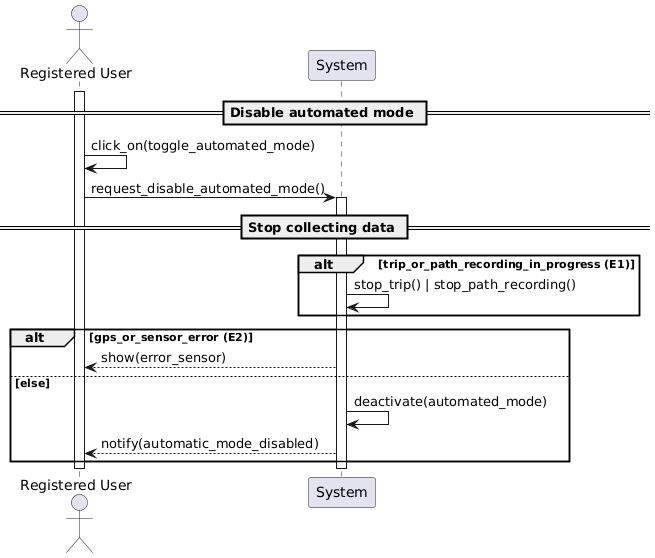
\includegraphics[width=\textwidth]{Images/Diagrams/Sequence/disable_auto_mode.png}
\caption{\label{fig:squencediagram}Sequence diagram for disable automated mode.}
\end{figure}

\pagebreak

\item \textbf{Record a Path in Manual Mode}

\begin{figure}[H]
\centering
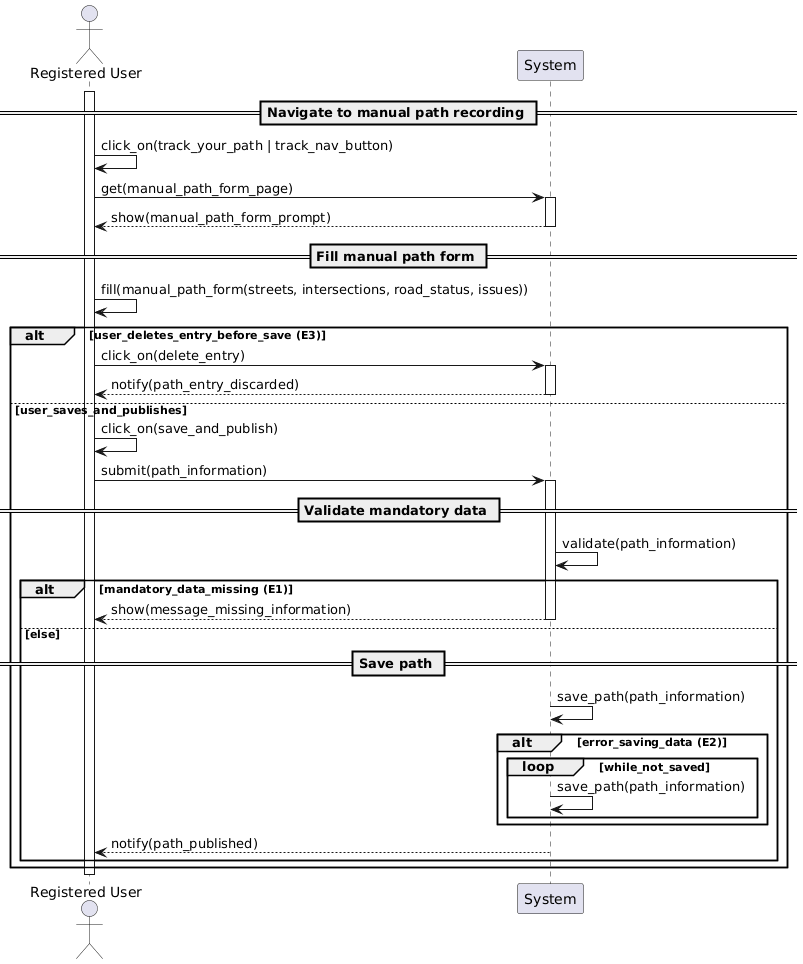
\includegraphics[width=\textwidth]{Images/Diagrams/Sequence/publish_path_manual_mode.png}
\caption{\label{fig:squencediagram}Sequence diagram for record a path in manual mode.}
\end{figure}

\pagebreak

\item \textbf{Record a Path in Automated Mode}

\begin{figure}[H]
\centering
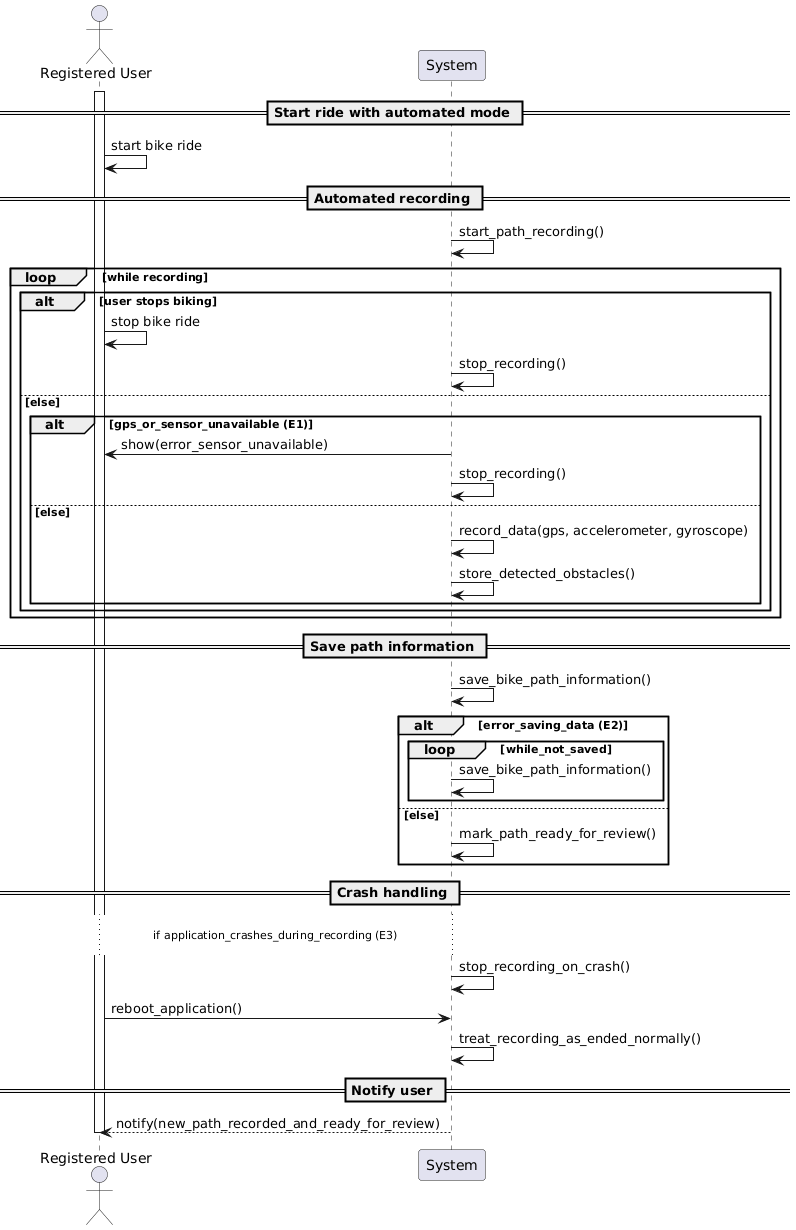
\includegraphics[scale=0.5]{Images/Diagrams/Sequence/record_path_automated.png}
\caption{\label{fig:squencediagram}Sequence diagram for record a path in automated mode.}
\end{figure}

\pagebreak

\item \textbf{Publish a pre-recorded automated mode path}

\begin{figure}[H]
\centering
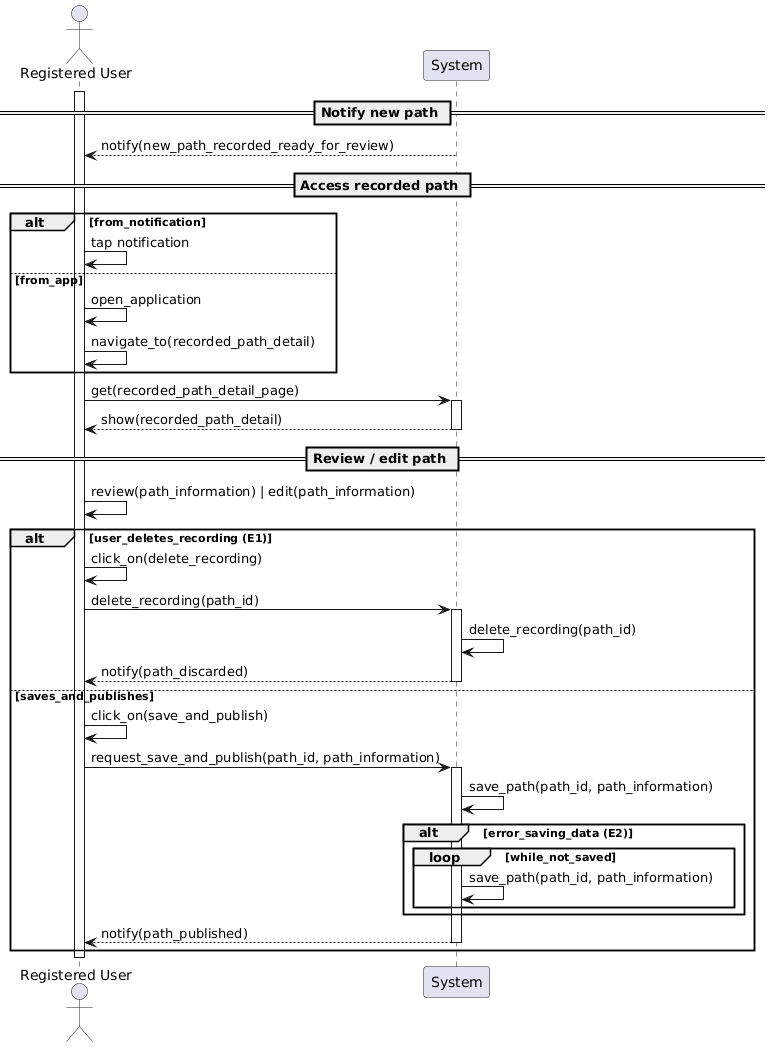
\includegraphics[width=\textwidth]{Images/Diagrams/Sequence/publish_path_auto_mode.png}
\caption{\label{fig:squencediagram}Sequence diagram for publish a pre-recorded automated mode path.}
\end{figure}

\pagebreak

\item \textbf{Logout}

\begin{figure}[H]
\centering
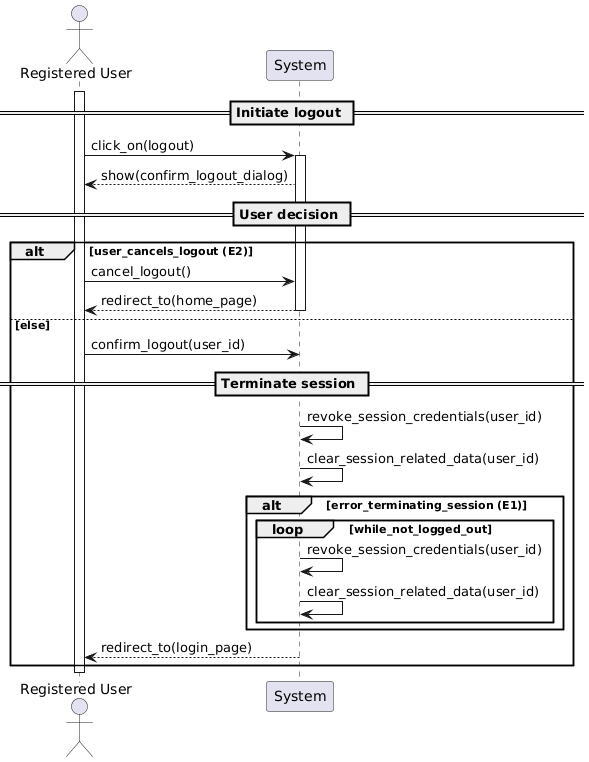
\includegraphics[width=\textwidth]{Images/Diagrams/Sequence/logout.png}
\caption{\label{fig:squencediagram}Sequence diagram for logout.}
\end{figure}

\pagebreak



\end{enumerate}

\subsection{Performance Requirements}
The system must be designed to handle a large number of concurrently connected and registered users, making scalability one of its primary functional requirements. As the platform is expected to serve many users at a time from many devices, it must be able to expand seamlessly while keeping performance degradation to a minimum. In other words, despite the number of users that use the different functionalities of the System, this still has to be reliable and stable.

Availability is equally essential: due to one of the functionality of the system being a "searching for paths" one, the uptime must be maximized and deliver information rapidly and efficiently. Key features such as search, tailored paths, and publishing processes must guarantee low response times and avoid introducing operational bottlenecks in such events, especially at peak of requests and high number of paths submitted. In addition, the system must support the upload and management of substantial volumes of metadata of the user paths, without compromising responsiveness or stability in the publish processing, but even when the automated mode is activated and user (taken account it is registered) is currently riding. 

Furthermore, any possible estimation of active users on the platform is hard to get, as there are many competitors that deals only with specific functionalities of BBP. To give an example, if we consider Strava's platform that deals with trip metrics, there are estimation of around 40-50 millions monthly users ~\cite{StravaYearInSport2025}. So, as a simple comparison (that takes account the part that gather trip information), BBP is supposed to cope with a number of concurrent users around 30.000, assuming an hypothetical average of two hours of usage per access. However, it is also reasonable to state that this estimation does not take account of the variance of such values, as there might be periods of the year with much greater accesses, and others with smaller ones. As a result, usage cannot be considered exclusively stable but, instead, a value that might oscillate. 

\subsection{Design Constraints}
\subsubsection{Standards compliance}
{Conformity Standards}
\begin{enumerate}
\item GDPR: The system should manage user data, location tracking and data path in the European Union, thus it is compliant with the General Data Protection Regulation according to the European guidelines.
\item Local privacy laws: The System should manage user data, location tracking and data path, thus it is compliant with the local laws in countries outside the European Union.
\item ISO/IEC 27001 ~\cite{ISOIEC27001}: The system must adopt structured and comprehensive information security management, in order to protect sensitive information and be adaptable to new risks.
\item ISO/IEC 25010 ~\cite{ISOIEC25010}: The system must be developed as to follow proper quality standards for reliability, performance, maintainability, and security.
\end{enumerate}
{Development Standards}
\begin{enumerate}
\item ISO/IEC 12207 ~\cite{ISOIECIEEE12207}: The system must apply the best practices in all the main processes that bring to its realization, in full compliant with the software life-cycle management standards.
\end{enumerate}
\subsubsection{Hardware Limitation}
\begin{enumerate}
\item In order for the application to work properly, the devices must be able to allocate enough resources to the background processes. In other words, a good CPU and enough RAM are needed. Minimum requirements like a quad-core processor is needed as a reliable resource for background activities. Furthermore, 4 GB of Ram is needed but for multi-tasking processes more of that is suggested. Long paths, especially for those taking hours, might affect the battery life-cycle of the device, especially if the automated mode is activated, as the usage of sensors is highly expensive in terms of battery consumption. As a result, battery devices shall be recent or have high volume capacity in order to avoid any early shutdown, leading the device to shut down the ongoing path data collection. 
\item Sensors, especially for the automated mode, are strictly necessary such as, gyroscopes, GPS sensors or even GNSS equivalent and accelerometer. Drivers shall be updated in order to use properly those sensors. 
\item In terms of software requirements, devices must provide the rights to the application to use most of the features in background in order to collect data of the path, as mentioned before. As a result, only latest versions of OS should be considered. However, as minimal requirements, in terms of Android Environment, require Android 10, that supports foreground-services and location authorizations in background, as might be limited in previous versions. For similar reasons, even in Apple environment, a minimum iOS version must be considered, by considering iOS 13, as it provides improved location tracking in background.
\item In terms of data collection, the System collects all the user data and the related path. As a result, the System should be able to  provide consistency and reliability in terms of paths scores and analysis. This is because, a good DBMS, especially an hybrid one, provide a good mixture of qualities of relational and non-relational models, as the System has to deal with different types of data, and concurrently also provide flexibility and high responsiveness.
\end{enumerate}

\subsubsection{Any other constraint}

In terms of connectivity, devices should rely on wireless infrastructures in order to send and receive data in case of collection of data, search and publication of paths. So, this is mostly an external party that affects, however, the user experience of the application as an overall. 

\subsection{Software System Attribute}
The BBP system must satisfy several key software attributes to ensure reliability, usability, and overall performance.     
\subsubsection{Scalability}
The most critical element is scalability as the system must efficiently handle a large number of registered and anonymous users simultaneously. In fact, the most costly effort is to decrease as much as possible the performance degradation even under peak usage. The system should manage new user registration and any surge of signs up. So the systems as a overall is supposed to be well efficiently structured.
\subsubsection{Availability}
As a result of Scalability, Availability is even crucial. The Search mode for bike paths requires to handle many sets of data already stored and organized in schema by the DBMS. As a result, the system must remain responsive and accessible at all times, delivering information quickly even at the highest peak of usage. Not to mention that the system must also provide robustness and fault tolerance. So, the system has to ready and able to manage many accesses at a time. If we consider periods of time when weather is especially suitable for riding, we expect to have peak of usage in the late morning (9:00 - 12:00) and late afternoon (17:00 - 20:00) between April and September. BBP is expected to be available, accessible and ready.
\subsubsection{Reliability}
The system should rely on a robust backup and recovery infrastructure capable of preserving data integrity at all times, even in the presence of unexpected faults. All critical elements must exhibit high reliability, so the architecture should incorporate redundant and parallelized components, ensuring that the failure of a single node, service, or storage unit does not compromise the availability of the platform.
\subsubsection{Security and privacy}
 Security is particularly important in terms of paths that are not directly related to the users, once published. Sensitive information must be stored and transmitted securely respecting user anonymity. In fact, data must be well stored and restricted accessed, preventing backdoor access and similar events. Furthermore, as GPS location is essential in the automated mode, user privacy is one of the most important aspect to mention. Given the sensitive nature of the information handled such that, every piece of user-related data must be protected with modern, robust cryptographic techniques. Only algorithms that are still considered secure by current standards should be used, such as hashing functions with adequate resistance like SHA-256, and encryption schemes such as AES-256 to safeguard stored content. 
 \subsubsection{Maintainability}
 In order to update the system in future and take account of additional new features, maintainability is then crucial, as well as an structured modular architecture. Furthermore, even a documentation for the related code should be clear, complete and easy to those in charge to maintain the system in future. Additionally, the project should adopt standard development practices such as version control workflows ( such as Git flow), automated testing, continuous integration/continuous delivery (CI/CD), and coding style guidelines. These practices reduce technical debt, improve code quality, and make sure that updates can be introduced safely and efficiently.
 \subsubsection{Portability}
 The system should be designed to be accessible and installed on operating systems such as iOS and Android. As a result, all the designed features should be all available, independently on the OS been used. Finally, the installation and update process should follow each platform’s best practices, ensuring seamless deployment via official app stores, secure updates, and minimal friction for the user.



%------------------------------------------------------------------------------------------------------------------------------------------------
\clearpage
{\color{Blue}{\section{Formal Analysis Using Alloy}}}
\label{sect:alloy}
\subsection{Alloy code}
G1 — Users can register and have a profile in BBP

This goal ensures that the system correctly manages user identities and registration.
The assertion \textit{differentUsersCannotBeSameUser} checks the uniqueness of users, stating that two distinct user instances cannot represent the same logical user. This prevents identity collisions within the system.

The assertion \textit{userRegisteredNotAnonymous} verifies that every registered user is not anonymous. In other words, once a user is registered, both must be associated with a concrete and identifiable profile. Moreover, these assertions guarantee that users in BBP are uniquely identifiable, non-anonymous once registered, and consistently represented throughout model phases.

G2 — Manual path creation

This goal concerns the manual creation of paths by users. The predicate \textit{showPath} models the evolution of the system state. So, initially, no trips are present. Eventually, two trips exist, representing the successful creation and storage of paths. This temporal behavior validates that manual path creation leads to persistent system state changes, confirming the goal. Trips are chosen on the select phase. 

G3 — Automatic path creation

This goal ensures that automatic and manual path creation are mutually exclusive.
The assertion \textit{AutomatedXorManual} expresses an 'exclusive-or' between the two modes. Specifically, if a data w is equal to Automated and at the same time equal to \textit{p.Recorded}, then it must not be equal to Manual. Furthermore, if w is equal to Manual and equal to \textit{p.Recorded}, then it must not be equal to Automated. This allows that a recorded path cannot either automatically and manually created at the same moment. The Alloy analyzer confirms this behavior by finding no counterexamples, meaning the constraint is consistent.

G4 — Browsing and viewing paths

The function \textit{searchPath} retrieves all paths composing a given trip, that it is constrained strictly to 1 by the facts. The predicate \textit{selectPath} calls the function and it ensures that at least one path is available for selection. This confirms that the system can search, retrieve, and select paths corresponding to user-defined criteria, fulfilling the browsing requirement. 

G5 — Recording and storing trips

The function \textit{extractTrip} ensures that each user is associated with at most one trip at a time. The predicate \textit{viewTrip} models the transition from no trips to one trip. These constraints validate that trips are correctly going through the phases, uniquely associated with users, and persist in the system.

G6 — Trip statistics and weather conditions

The predicate \textit{viewTripAtCheckInfo} ensures that a trip eventually exists. Then the trip reaches the \textit{CheckInfo} situation. The trip belongs to the requesting user. This verifies that statistical and contextual information is available and accessible for recorded trips.

G7 — Merging information and generating the optimal path

This goal describes the final phases of application usage, including information merging and path publication. The predicate \textit{show[]} models the evolution of the system over time. Initially, the number of Trip instances is 0, representing the state before any trip is created. At some intermediate point, the number of Trip instances becomes 3, representing multiple partial or candidate trips during processing. Finally, there exists a Trip whose situation is \textit{Publish}, representing the successful generation and publication of the optimal path. Overall, this goal captures the intended steps of the application, from initial usage, through intermediate processing steps, to the final publication of a single optimal trip of a given user.

\begin{lstlisting}[
    style=alloy,
]

abstract sig Status {}
one sig Optimal, Acceptable, Sufficient, Difficult extends Status {}
abstract sig Way{}
one sig Automated, Manual extends Way{}
sig idUser {}
sig idPath{}
sig idTrip{}

enum currentSituation {
		Search, 
		Select, 
		Ride, 
		CheckInfo, 
		Publish
}

var sig Trip {
	var id: one idTrip,
	var ComposedOf: one Path, 
	var BelongingTo: one System,
	var userRelated: one user,
	var situation: one currentSituation
} {
	#ComposedOf = 1
}

sig user {
	id: one idUser,
	var tripInfo: lone Trip
} {
}

sig userAnonymous extends user {
}

sig Path {
	id: idPath,
	var PartOf: set Trip,
	Recorded: one Way,
 	computedStatus: one Status      
} {
}

one sig System {
	ProvidingPaths: set Path,
	toUser: some user
}{	
}

------------------------------ facts on step progression ------------------------------


// Every situation is a ordered step
fun nextSituation[t: Trip]: one currentSituation {
	(t.situation = Search) => Select else
	(t.situation = Select) => Ride else
	(t.situation = Ride) => CheckInfo else
	(t.situation = CheckInfo) => Publish else
	(t.situation = Publish) => Search else none
}

// Recall nextSituation function in order to move along steps
fact stateProgression {
	always (
		all t: Trip |
				t.situation' = t.situation or
 				t.situation' = nextSituation[t] or
 				t not in Trip'
 	)
}

// Every steps appears at select
fact insertingTrip {
	always (
		all t: Trip | 
			once (t.situation = Select) 
	)
}

// Trip rules along steps
fact finalizingTrip {
	always (all t: Trip |  after t.situation = CheckInfo implies eventually (t not in Trip))
	always (all t: Trip | t not in Trip' implies after always t not in Trip')
}

// Trip can't disappear if appears at least once after select
fact persistencyAlongSteps {
  all t: Trip| all cS: t.situation | 
    (cS = Search or cS = Select or cS = Ride or cS = CheckInfo ) implies
      always (t in Trip')
}

fact persistencyPathAlongSteps {
	all t: Trip, s: System | s in t.BelongingTo implies always (s in t'.BelongingTo)
	all t: Trip, u: user | u in t.userRelated implies always (u in t'.userRelated)
	all t: Trip, p: Path | p in t.ComposedOf implies always (p in t'.ComposedOf)
	all t: Trip, idt: idTrip | idt in t.id implies always (idt in t'.id)
}

fact userPersistency {
	user = user' 
}

fact userOfTripRemainsSame {
    always all t: Trip | t'.userRelated = t.userRelated
}

// all user have a unique email address and a unique username
fact uniqueID{
	always ( all disj u1 , u2 : user | u1.id != u2.id )
}

// every Email is associated to one User
fact uniqueID {
	always ( all i : idUser | one u : user | u.id = i )
}
------------------------------------------------------------------------------------------------------

// Relationship between Trip, path and userAnonymous
fact {
	no u: userAnonymous | all t: Trip | all p: Path | p in t.ComposedOf and t in u.tripInfo
}

fact {
	all u: user | all s: System | u in s.toUser
}

fact {
	all t: Trip | all u: user | u in t.userRelated implies (t in u.tripInfo)
}

fact {
	all i: idUser | all u: user | all u2: user | i in u.id and u != u2 implies always(i not in u2.id)
}

// users must appear and be related to trip
fact  {
	all t: Trip | all u: user | u = t.userRelated implies (no t2: Trip | t2 != t and u in t2.userRelated)
	all t: Trip | all u: user | u = t.userRelated implies (no t2: Trip' | t2 != t and u in t2.userRelated)
	all t: Trip | all u: user | u = t.userRelated implies after always (no t2: Trip | t2 != t and u in t2.userRelated)
	all u: user | all t: Trip | u = t.userRelated implies always (t in u.tripInfo)
}

fact  {
	always( all u1: user | all t: Trip | all s: System | t in u1.tripInfo implies (u1 in t.userRelated and u1 in s.toUser and t.ComposedOf in s.ProvidingPaths))
}

fact {
	always(all disj t1, t2: Trip | t1.id != t2.id )
}

fact {
    all t: Path | t.id' = t.id
}

fact userTripHasPath {
	always (all t: Trip | all u: user | t in u.tripInfo implies (all p: Path | p in t.ComposedOf))
}

fact {
	always(all an: userAnonymous | all u: user | an != u)
}

fact {
	all u1, u2: user | all t: Trip | t in u1.tripInfo and u1.id != u2.id implies (t not in u2.tripInfo)
}

// user is quantifiable and unique
fact distintUser {
	all u1, u2: user | u1.id != u2.id iff (u1 != u2)	
	all u1, u2: user | u1 != u2 implies after always u1 != u2		
}

fact {
	all t1, t2: Trip | t1 != t2 implies  t1.id != t2.id
	all t1, t2: Trip | t1 != t2 implies after always t1.id != t2.id
}

// future steps must have same patters of previous steps
fact {
	(all sys: System | all t: Trip | all u: user | sys in t.BelongingTo and u in t.userRelated and t in u.tripInfo and u in sys.toUser implies after always ( System' = t.BelongingTo and user' = t.userRelated and user' = sys.toUser and Trip' = u.tripInfo))
}

-----------------------------------------------------------------------------------------------------

// G1: Users can register and have a profile in BBP application.

assert differentUsersCannotBeSameUser {
 	all u1, u2: user | u1.id  != u2.id implies u1 = u2
}

assert userRegisteredNotAnonymous {
	all u: user | all an: userAnonymous | u = user implies u != an
}

// G2: Users manually create bike paths in an inventory by specifying the name of the streets and the status.

pred showPath {
#Trip = 0
eventually (#Trip = 2) 
}

// G3: Users create bike paths in an automated mode where the system acquire data from the user's mobile device and reconstruct the path.

assert AutomatedXorManual {
	all w: Way | all p: Path | w = Automated and w =  p.Recorded implies (w != Manual)
	all w: Way | all p: Path | w = Manual and w = p.Recorded implies (w != Automated)
}

// G4: Users browse bike paths within the inventory. They can specify an origin and destination and ask the system to visualize the bike path on a map.

fun searchPath[t: Trip]: set Path{
	{
		p: Path | some g: t.ComposedOf | p = g
	}
}

pred selectPath[t: Trip]{
	some searchPath[t] 
}

// G5: Users record their trips and store them to keep track of their cycling activities.

fun extractTrip[u: user]: lone Trip {
    u.tripInfo
}

pred viewTrip [u: user] {
	#Trip = 0
	eventually (#Trip = 1) 
	#extractTrip[u] <= 1
}

// G6: Users can see for a recorded trip various statistical data of the user performances as well as meteorological information during the respective trip.

pred viewTripAtCheckInfo[u: user] {
    #Trip = 0
	eventually ( some t:Trip | #Trip = 1 and t.situation = CheckInfo and  t in u.tripInfo ) 
}

// G7: The system uses information published by the users about the paths by merging pieces of information to generate the optimal path, using the freshness and number of confirmed data.

pred show[] {
    #Trip = 0
    eventually (#Trip = 3) 
    eventually (some t: Trip | t.situation = Publish)
}

//check differentUsersCannotBeSameUser for 2 but exactly 3 user
//check userRegisteredNotAnonymous  for 3 but exactly 3 user
//check AutomatedXorManual for 2
//run viewTripAtCheckInfo for 3 but exactly 3 user
//run showPath for 3 but exactly 3 user
//run viewTrip for 3 but exactly 3 user
//run selectPath for 3 but 1 Path, 5 steps
//run show for 3 but exactly 3 user

\end{lstlisting}

\newpage
\begin{figure}
    \centering
    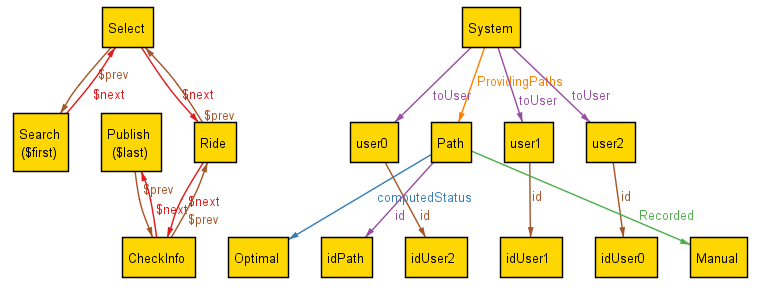
\includegraphics[width=0.5\linewidth]{RASD/Images/imagesAlloy/idleSearchPhase.png}
    \caption{Idle phase}
    \label{fig:placeholder}
\end{figure}

\begin{figure}
    \centering
    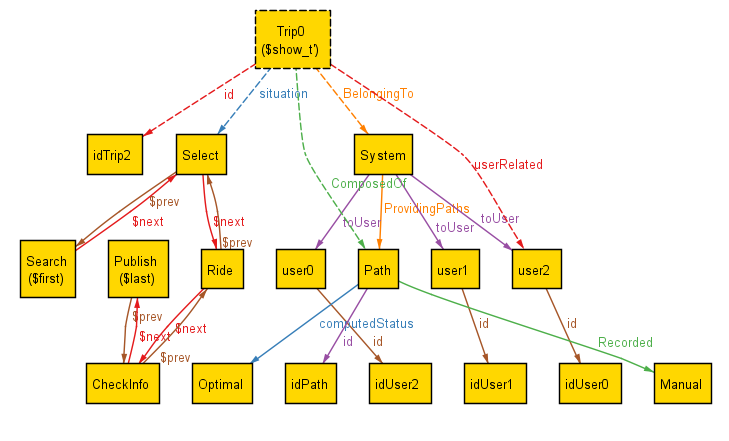
\includegraphics[width=0.5\linewidth]{RASD/Images/imagesAlloy/Select.png}
    \caption{Select Phase}
    \label{fig:placeholder}
\end{figure}

\begin{figure}
    \centering
    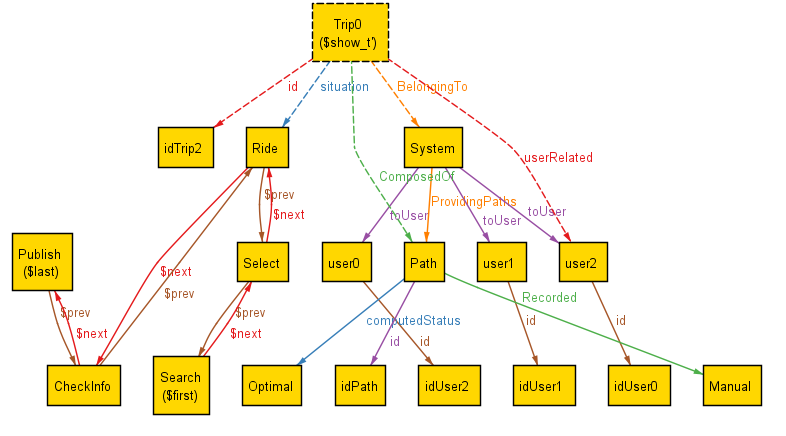
\includegraphics[width=0.5\linewidth]{RASD/Images/imagesAlloy/Ride.png}
    \caption{Ride phase}
    \label{fig:placeholder}
\end{figure}

\begin{figure}
    \centering
    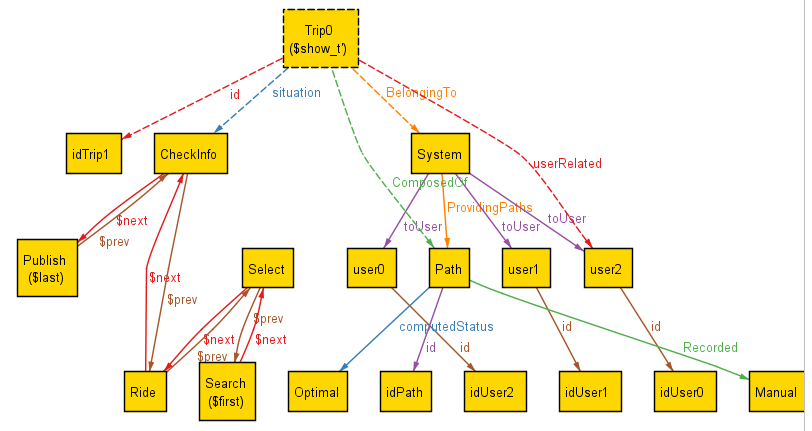
\includegraphics[width=0.5\linewidth]{RASD/Images/imagesAlloy/CheckInfo.png}
    \caption{Checkinfo phase}
    \label{fig:placeholder}
\end{figure}

\begin{figure}
    \centering
    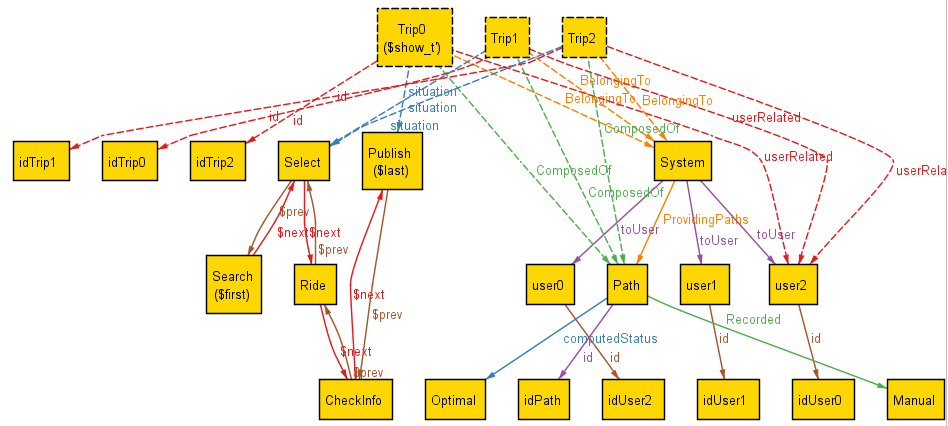
\includegraphics[width=0.5\linewidth]{RASD/Images/imagesAlloy/PublishPhase.png}
    \caption{Publish phase}
    \label{fig:placeholder}
\end{figure}

%------------------------------------------------------------------------------------------------------------------------------------------------
\clearpage
{\color{Blue}{\section{Effort Spent}}}
\label{sect:effort}
The following table displays the number of hours each group member spent on the various sections of the document.


\begin{table}[ht]
\begin{tabular}{|l|c|c|c|c|}
\hline
\textbf{Group members}      & \multicolumn{1}{l|}{\textbf{Chapter 1}} & \multicolumn{1}{l|}{\textbf{Chapter 2}} & \multicolumn{1}{l|}{\textbf{Chapter 3}} & \multicolumn{1}{l|}{\textbf{Chapter 4}} \\ \hline
Alessandro Barbera & 2                              & 8                              & 22                              & 1                              \\ \hline
Nicolas Bolanos    & 4                              & 11                              & 8                              & 12                              \\ \hline
Massimiliano Nuzzo & 1                              & 3                              & 5                              & 25                              \\ \hline
\end{tabular}
\end{table}

{\color{Blue}{\section{Use of Generative AI}}}
\label{sect:genAI}
\subsection{Use of Generative Artificial Intelligence Tools}

Generative Artificial Intelligence (AI) tools were employed to support various stages of the documentation and design process in this project. The tools used include \textbf{Perplexity AI} and \textbf{Gemini}, selected for their advanced natural language generation and reasoning capabilities. These tools assisted in tasks related to technical writing, software modeling, and language revision, always under careful human supervision and validation.

\textbf{All strategic and main decision processes were entirely human-driven}. AI served strictly as a tool to augment these decisions, automate routine work, and save time, without influencing core architectural or methodological choices.

The specific prompts provided to the AI systems were explicitly formulated to focus on technical and linguistic support. Examples of inputs include: 
\begin{itemize}
    \item ``Help me generate a PlantUML code Domain Class Diagram from the following Domain Class Diagram sketch.''
    \item ``Help me brainstorm goals for the following software use case.''
    \item ``Help me write in a formal way the following functional requirements.''
    \item ``Help me rewrite the following section for a software design document.''
    \item ``Help me look for grammar and spelling mistakes.''
\end{itemize}

The outputs obtained included automatically generated textual content such as structured PlantUML code for all diagrams, rewritten and polished technical documentation, formalized versions of functional requirements, and identified language corrections. In brainstorming tasks, the tools provided diverse options and design considerations that served as inspiration for choosing what to include in the document.

Verification, refinement, and integration of AI-generated outputs were performed systematically. Each generated segment was carefully reviewed before inclusion. For code artifacts (Alloy), outputs were tested directly within the target environment or modeling software to confirm proper functionality and consistency with the project's requirements. When AI responses incorporated external knowledge sources, these references were verified for accuracy and reliability before use. Sections of text that did not meet quality or factual standards were either revised or discarded entirely.

The integration of AI assistance enhanced productivity and coherence across the project documentation. It supported the generation of consistent technical descriptions and facilitated the refinement of complex technical ideas into well-structured prose. Human oversight remained indispensable; all final content (including diagrams, requirements, and textual documentation) was critically validated, edited, and approved by the authors to ensure academic rigor, correctness, and originality.

Overall, Generative AI tools functioned as an auxiliary mechanism for idea development, code drafting, and language improvement, rather than as a replacement for human analysis or authorship. Through responsible use and verification, these tools contributed to improving the clarity, precision, and quality of the final project deliverables.


%------------------------------------------------------------------------------------------------------------------------------------------------
\clearpage
\addcontentsline{toc}{section}{References}
\bibliographystyle{plain}
\bibliography{main}
%------------------------------------------------------------------------------------------------------------------------------------------------




\end{document}
